%%%%%%%%%%%%%%%%%%%%%%%%%%%%%%%%%%%%%%%%%
% Beamer Presentation
% LaTeX Template
% Version 1.0 (10/11/12)
%
% This template has been downloaded from:
% http://www.LaTeXTemplates.com
%
% License:
% CC BY-NC-SA 3.0 (http://creativecommons.org/licenses/by-nc-sa/3.0/)
%
%%%%%%%%%%%%%%%%%%%%%%%%%%%%%%%%%%%%%%%%%

%----------------------------------------------------------------------------------------
%	PACKAGES AND THEMES
%----------------------------------------------------------------------------------------

\documentclass{beamer}

\mode<presentation> {

% The Beamer class comes with a number of default slide themes
% which change the colors and layouts of slides. Below this is a list
% of all the themes, uncomment each in turn to see what they look like.

%\usetheme{default}
%\usetheme{AnnArbor}
%\usetheme{Antibes}
%\usetheme{Bergen}
%\usetheme{Berkeley}
%\usetheme{Berlin}
%\usetheme{Boadilla}
%\usetheme{CambridgeUS}
%\usetheme{Copenhagen}
%\usetheme{Darmstadt}
%\usetheme{Dresden}
%\usetheme{Frankfurt}
%\usetheme{Goettingen}
%\usetheme{Hannover}
%\usetheme{Ilmenau}
%\usetheme{JuanLesPins}
%\usetheme{Luebeck}
\usetheme{Madrid}
%\usetheme{Malmoe}
%\usetheme{Marburg}
%\usetheme{Montpellier}
%\usetheme{PaloAlto}
%\usetheme{Pittsburgh}
%\usetheme{Rochester}
%\usetheme{Singapore}
%\usetheme{Szeged}
%\usetheme{Warsaw}

% As well as themes, the Beamer class has a number of color themes
% for any slide theme. Uncomment each of these in turn to see how it
% changes the colors of your current slide theme.

%\usecolortheme{albatross}
%\usecolortheme{beaver}
%\usecolortheme{beetle}
%\usecolortheme{crane}
%\usecolortheme{dolphin}
%\usecolortheme{dove}
%\usecolortheme{fly}
%\usecolortheme{lily}
%\usecolortheme{orchid}
%\usecolortheme{rose}
%\usecolortheme{seagull}
%\usecolortheme{seahorse}
%\usecolortheme{whale}
%\usecolortheme{wolverine}

%\setbeamertemplate{footline} % To remove the footer line in all slides uncomment this line
%\setbeamertemplate{footline}[page number] % To replace the footer line in all slides with a simple slide count uncomment this line

%\setbeamertemplate{navigation symbols}{} % To remove the navigation symbols from the bottom of all slides uncomment this line
}

\usepackage{graphicx} % Allows including images
\usepackage{booktabs} % Allows the use of \toprule, \midrule and \bottomrule in tables
\usepackage{url}

%----------------------------------------------------------------------------------------
%	TITLE PAGE
%----------------------------------------------------------------------------------------
\title[Similarity Measures]{Evaluation of semantic similarity measures} % The short title appears at the bottom of every slide, the full title is only on the title page

\author{\underline{Maxat Kulmanov}, Robert Hoehndorf} % Your name
\institute[] % Your institution as it will appear on the bottom of every slide, may be shorthand to save space
{
King Abdullah University of Science and Technology, Saudi Arabia \\
Computational Bioscience Research Center \\
Bio-Ontologies Research Group% Your institution for the title page
\medskip
% \textit{maxat.kulmanov@kaust.edu.sa} % Your email address
}
\date{} % Date, can be changed to a custom date

\begin{document}

\begin{frame}
\titlepage % Print the title page as the first slide
\end{frame}

%----------------------------------------------------------------------------------------
%	PRESENTATION SLIDES
%----------------------------------------------------------------------------------------

%------------------------------------------------
\section{Introduction} % Sections can be created in order to organize your presentation into discrete blocks, all sections and subsections are automatically printed in the table of contents as an overview of the talk
%------------------------------------------------

%\subsection{Subsection Example} % A subsection can be created just before a set of slides with a common theme to further break down your presentation into chunks

\begin{frame}
\frametitle{Semantic Similarity Measures}
\begin{itemize}
\item Semantic similarity measures capture the strength of interaction between concepts based on their meaning.
\item Widely used in bioinformatics
\begin{itemize}
\item Protein-protein interaction identification
\item Gene-Disease associations
\item Patient diagnoses 
\end{itemize}
\end{itemize}
\end{frame}

%------------------------------------------------

\begin{frame}
\frametitle{Semantic Similarity Measures}
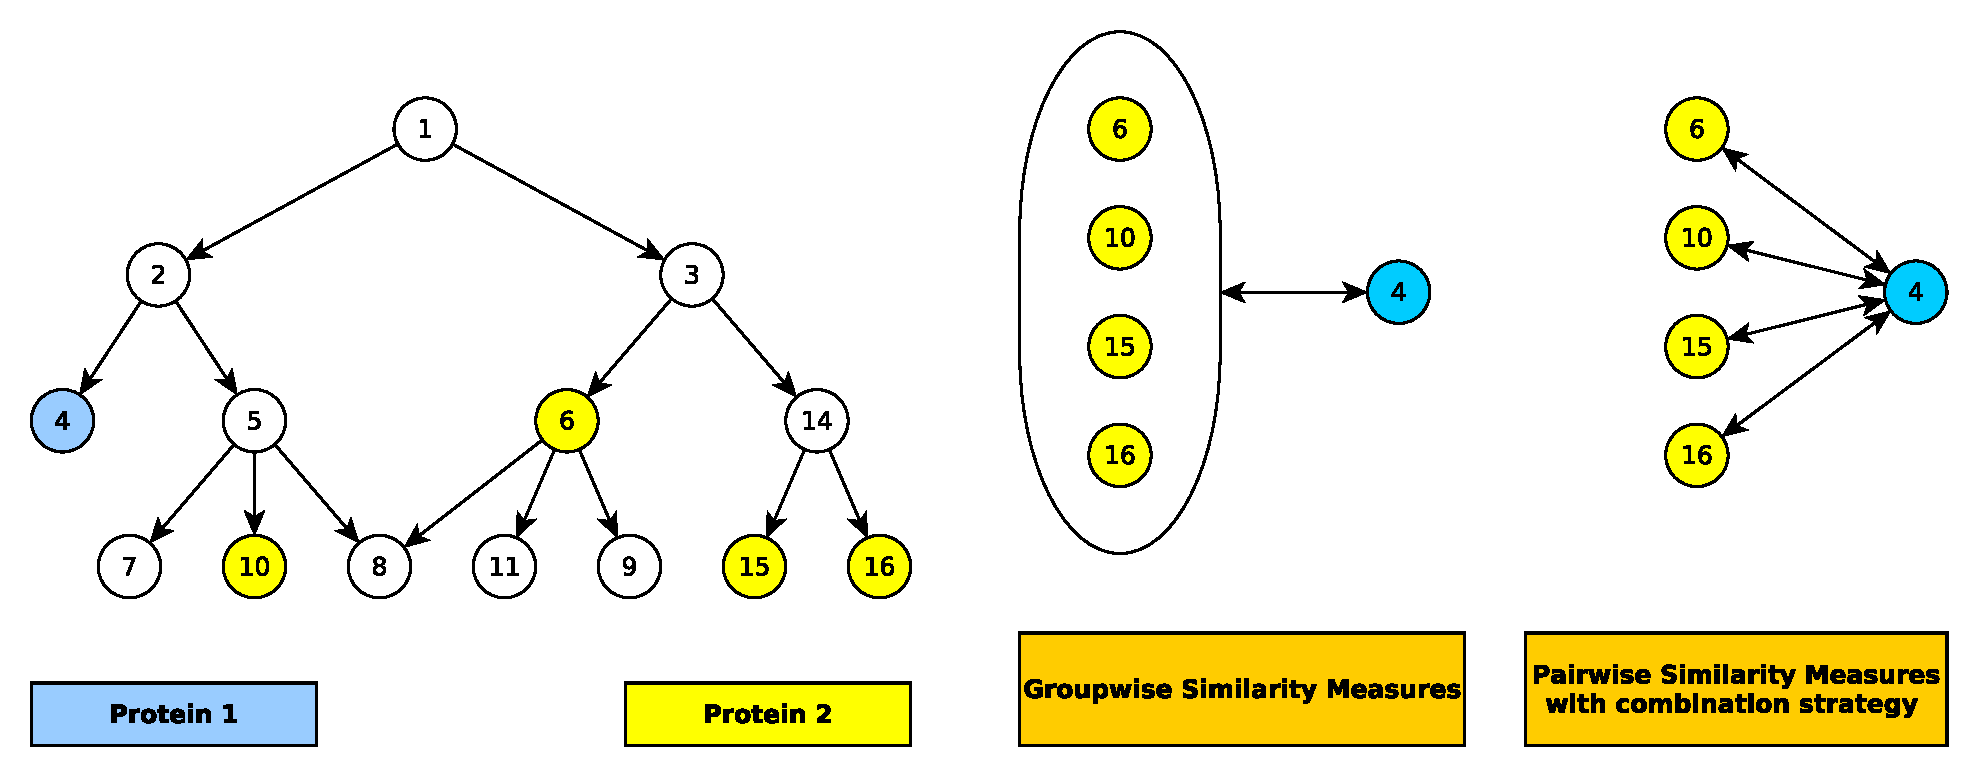
\includegraphics[width=1.0\linewidth]{figures/annots.pdf}
\end{frame}

%------------------------------------------------

\section{Motivation and Aim}

\begin{frame}
\frametitle{Motivation and Aim}
\begin{itemize}
\item Large number of semantic similarity measures has been developed:
\begin{itemize}
\item 21 groupwise
\item 38 pairwise with 7 different combination strategies
\item Available in Semantic Measures Library \url{http://www.semantic-measures-library.org/}
\end{itemize}
\item Classify semantic similarity measures by their sensitivity to the:
\begin{itemize}
\item number of annotated classes
\item difference of the number of annotated classes
\end{itemize}
\end{itemize}
\end{frame}

%------------------------------------------------

\section{Materials and Methods}

%------------------------------------------------

\begin{frame}
\frametitle{Materials}
\begin{itemize}
\item Gene Ontology (GO)
\item 6,108 gene annotations from Yeast Genome Database. Annotation sizes vary from 1 to 55
\item 5,500 randomly generated annotations
\begin{itemize}
\item 55 groups with 100 genes in each:
\begin{itemize}
\item 1st group annotated with 1 GO class
\item 2nd group annotated with 2 GO classes
\item 3rd group annotated with 3 GO classes
\item and so on
\end{itemize}
\end{itemize}
\end{itemize}

\end{frame}
%------------------------------------------------

\begin{frame}
\frametitle{Methods}
\begin{itemize}
\item Compute similarity between each pair of genes
\begin{itemize}
\item 18,656,886 similarity values for yeast annotations \\ ((6108 + 1) / 2 * 6108)
\item 15,127,750 similarity values for random annotations
\end{itemize}
\item Group similarities by annotations size 
\item Group similarities by annotations size difference
\item Take average similarities for all groups
\end{itemize}

\end{frame}

\section{Results}

\begin{frame}
\frametitle{Results}
\begin{itemize}
\item Sensitive
\begin{itemize}
\item Similarity value increases when annotation size (difference) increases
\item Similarity value decreases when annotations size (difference) increases
\end{itemize}
\item Not sensitive 
\end{itemize}

\end{frame}

\begin{frame}{Annotation size - Groupwise Similarity Measures}

\begin{figure}
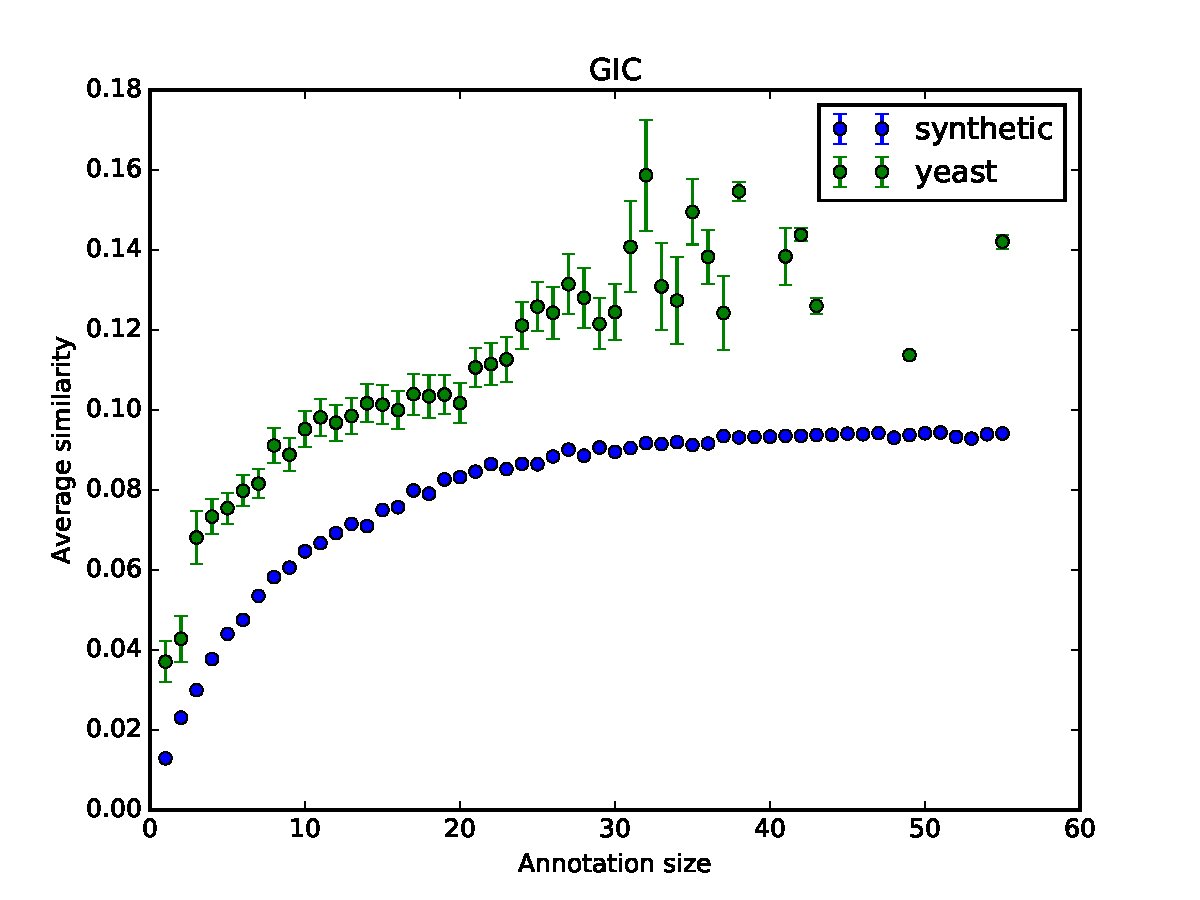
\includegraphics[width=0.5\linewidth, height=0.4\textheight]{groupwise/SIM_GROUPWISE_DAG_GIC_avg.pdf}
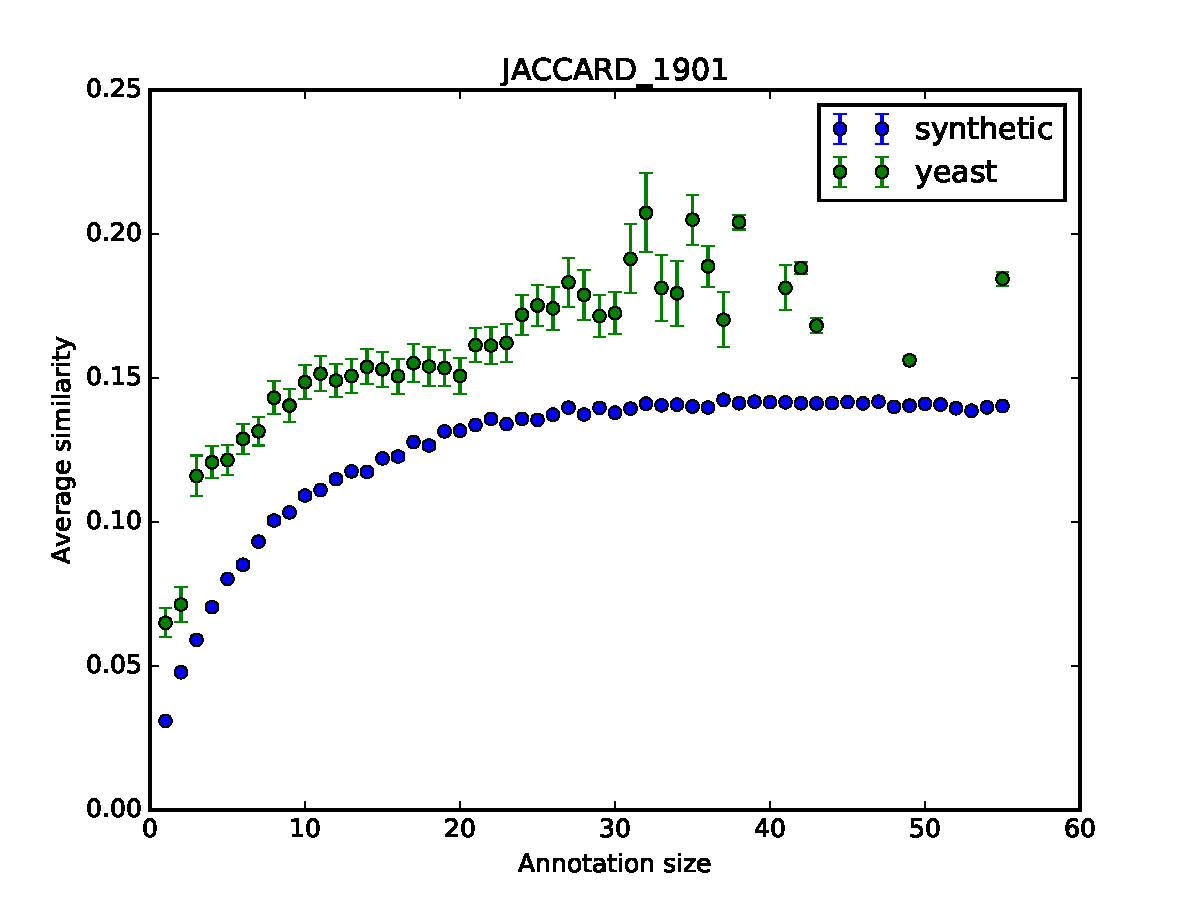
\includegraphics[width=0.5\linewidth, height=0.4\textheight]{groupwise/SIM_FRAMEWORK_DAG_SET_JACCARD_1901_avg.pdf} \\
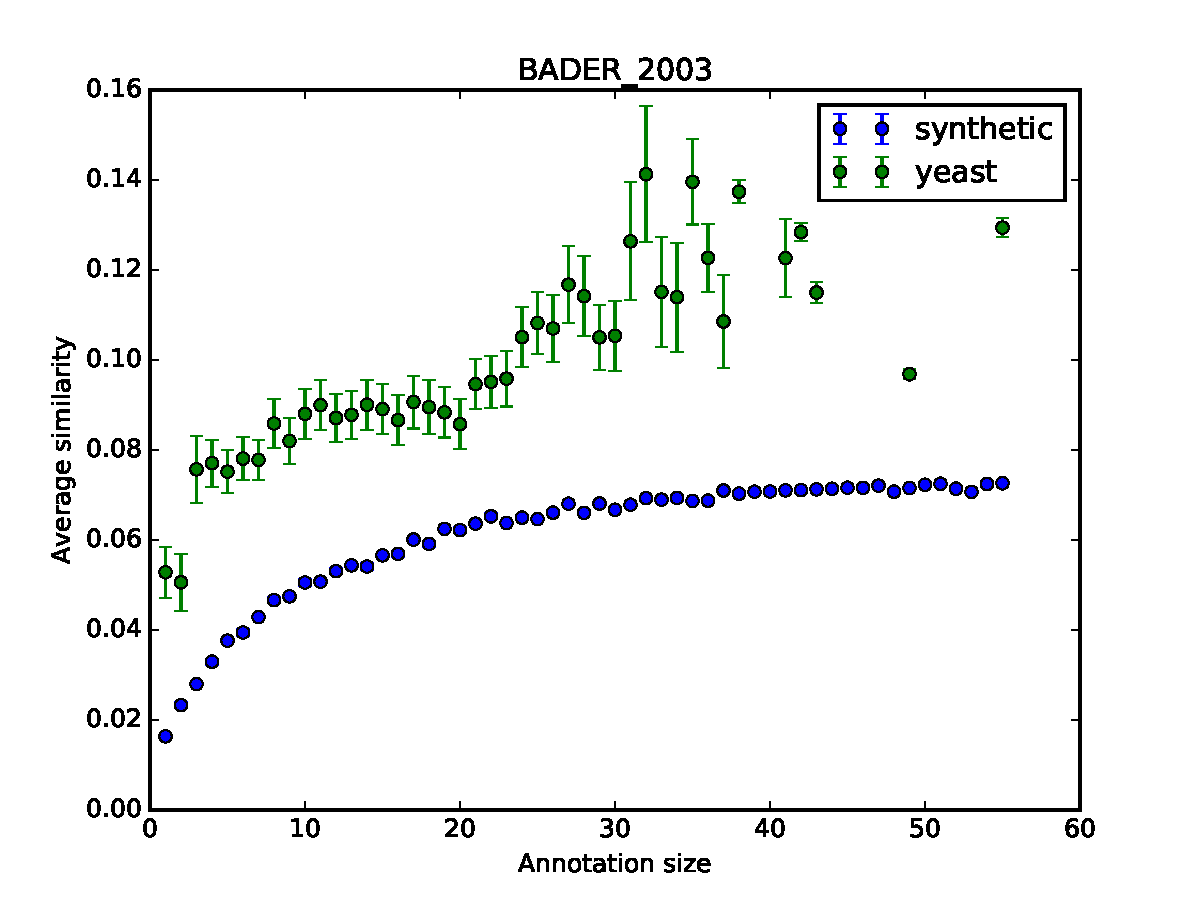
\includegraphics[width=0.5\linewidth, height=0.4\textheight]{groupwise/SIM_FRAMEWORK_DAG_SET_BADER_2003_avg.pdf}
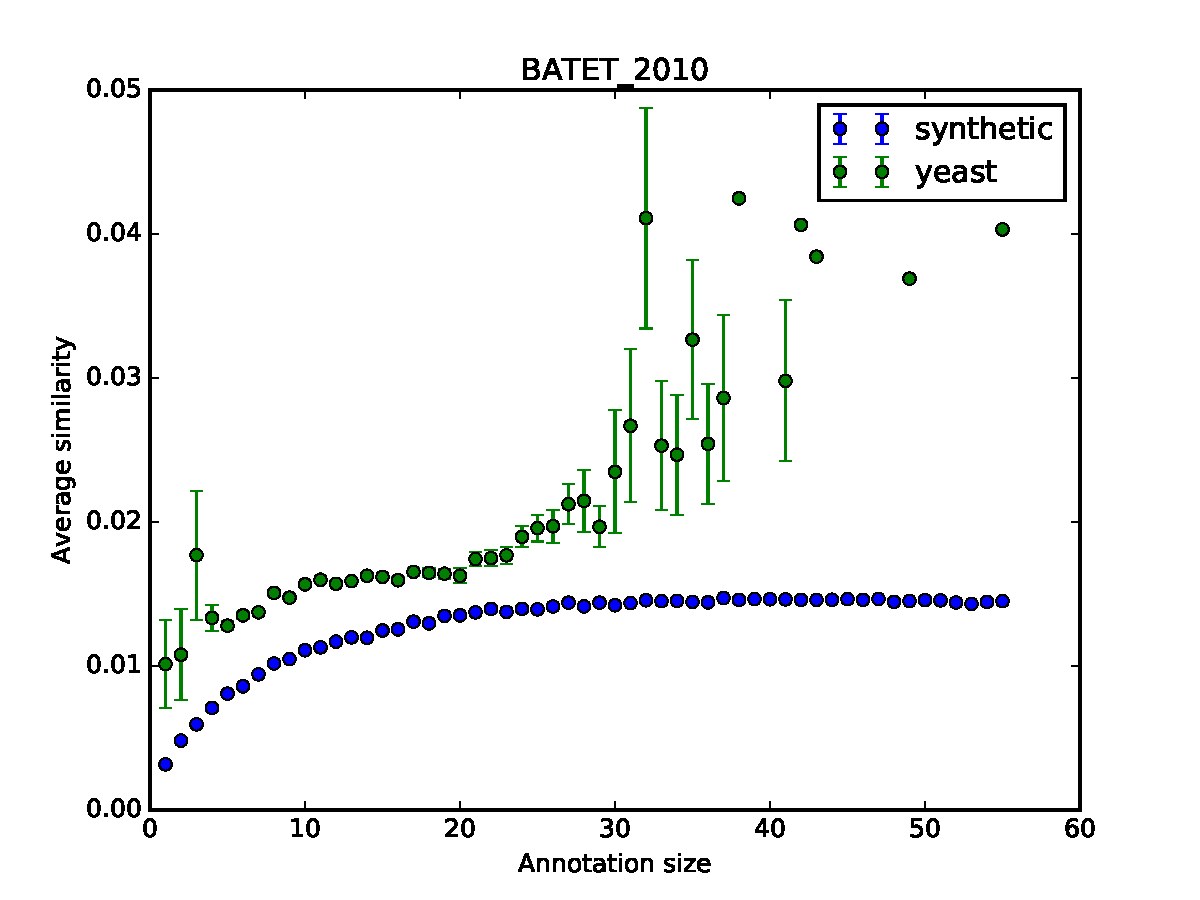
\includegraphics[width=0.5\linewidth, height=0.4\textheight]{groupwise/SIM_FRAMEWORK_DAG_SET_BATET_2010_avg.pdf} \end{figure}

\end{frame}


\begin{frame}{Annotation size - Groupwise Similarity Measures}

\begin{figure}
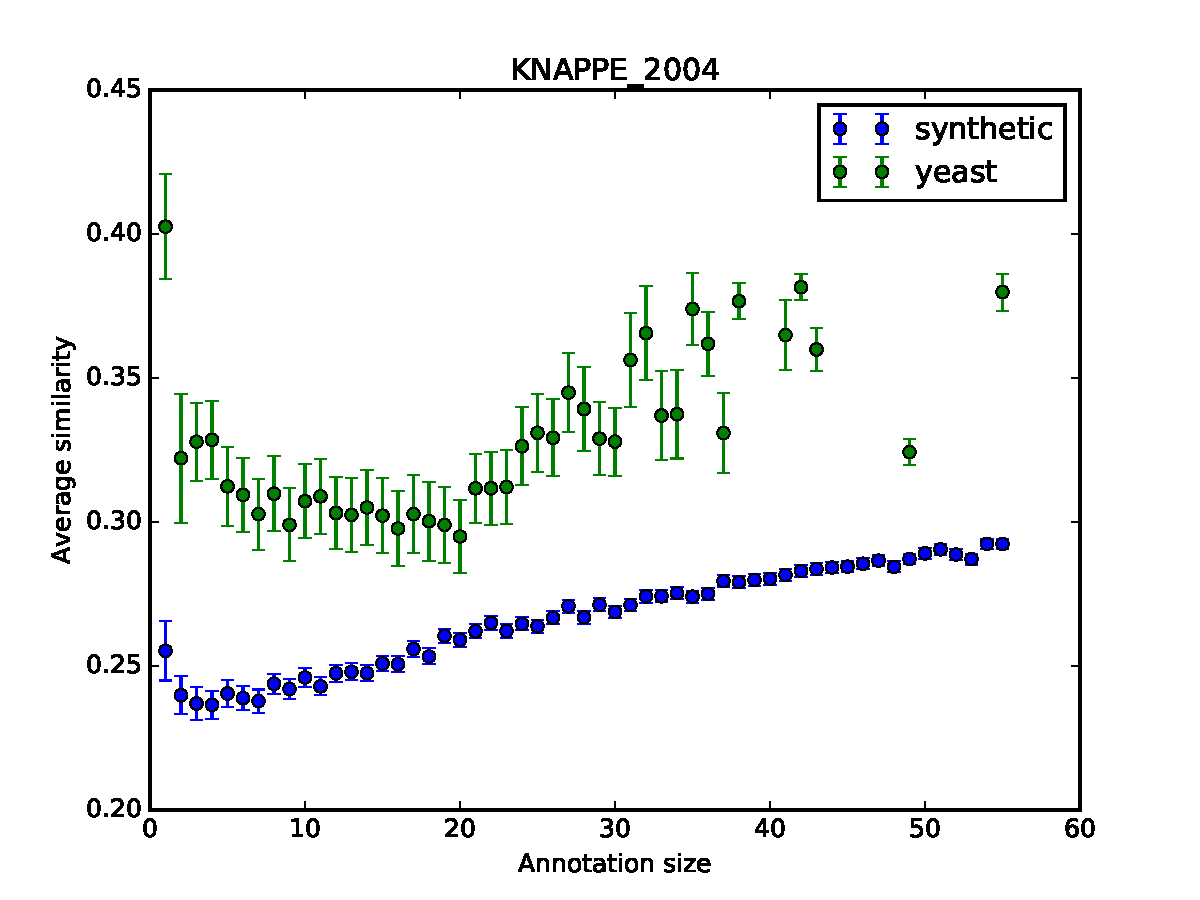
\includegraphics[width=0.5\linewidth, height=0.4\textheight]{groupwise/SIM_FRAMEWORK_DAG_SET_KNAPPE_2004_avg.pdf}
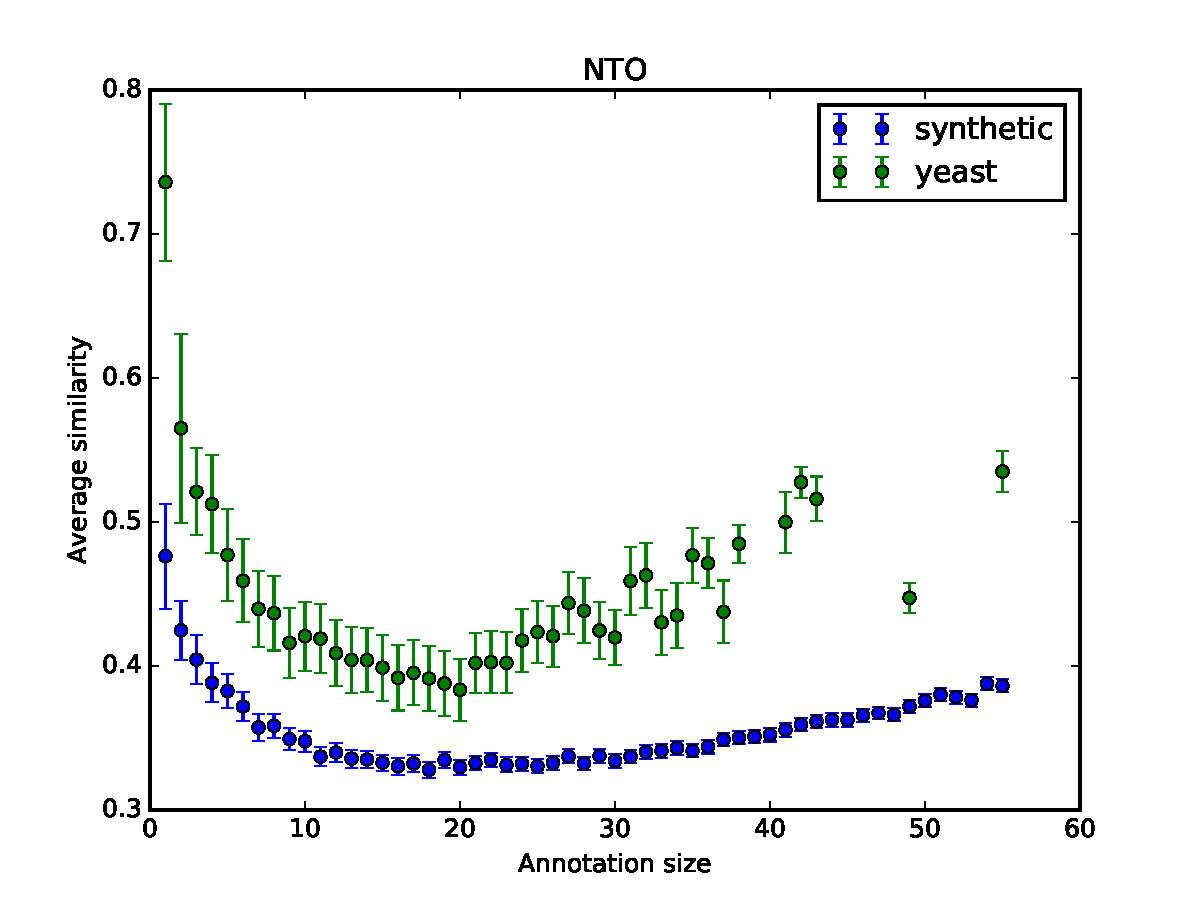
\includegraphics[width=0.5\linewidth, height=0.4\textheight]{groupwise/SIM_GROUPWISE_DAG_NTO_avg.pdf}\\
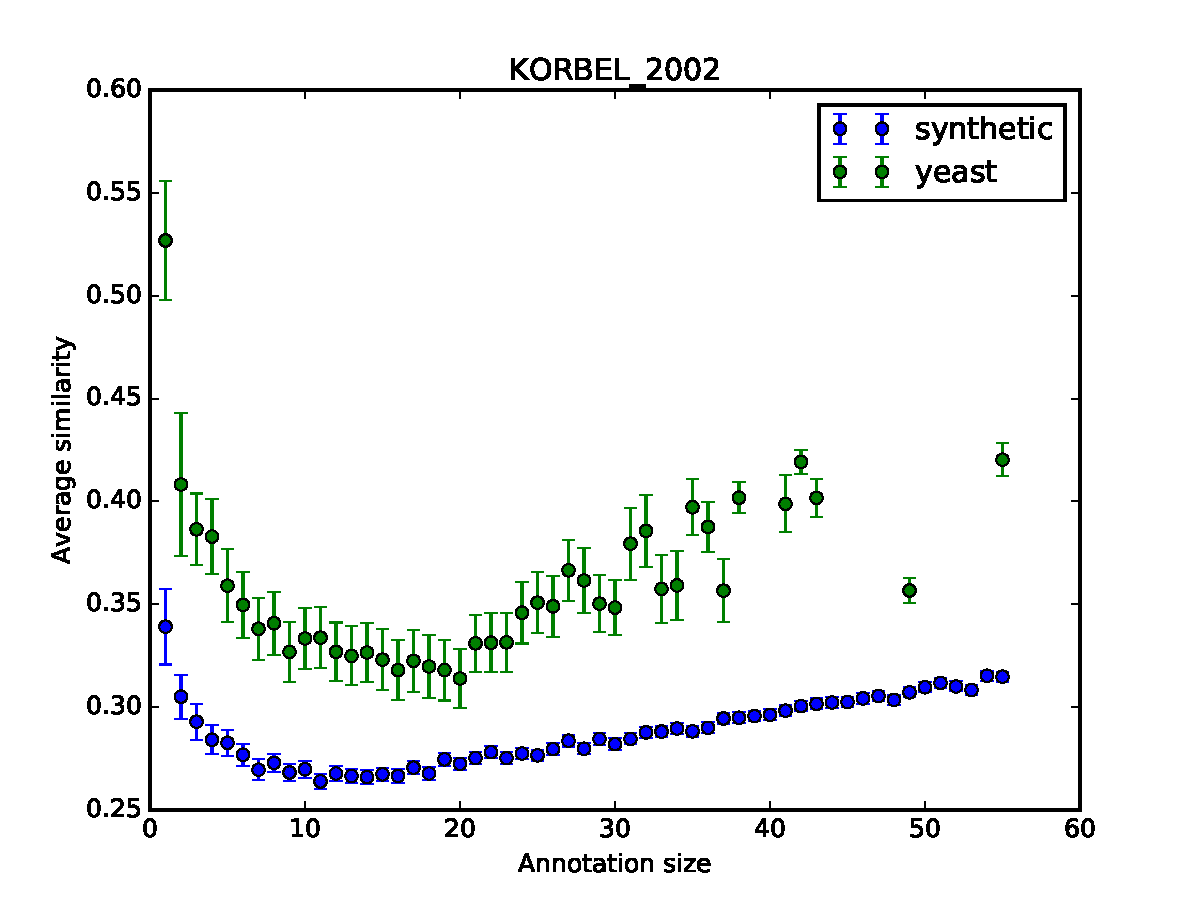
\includegraphics[width=0.5\linewidth, height=0.4\textheight]{groupwise/SIM_FRAMEWORK_DAG_SET_KORBEL_2002_avg.pdf}
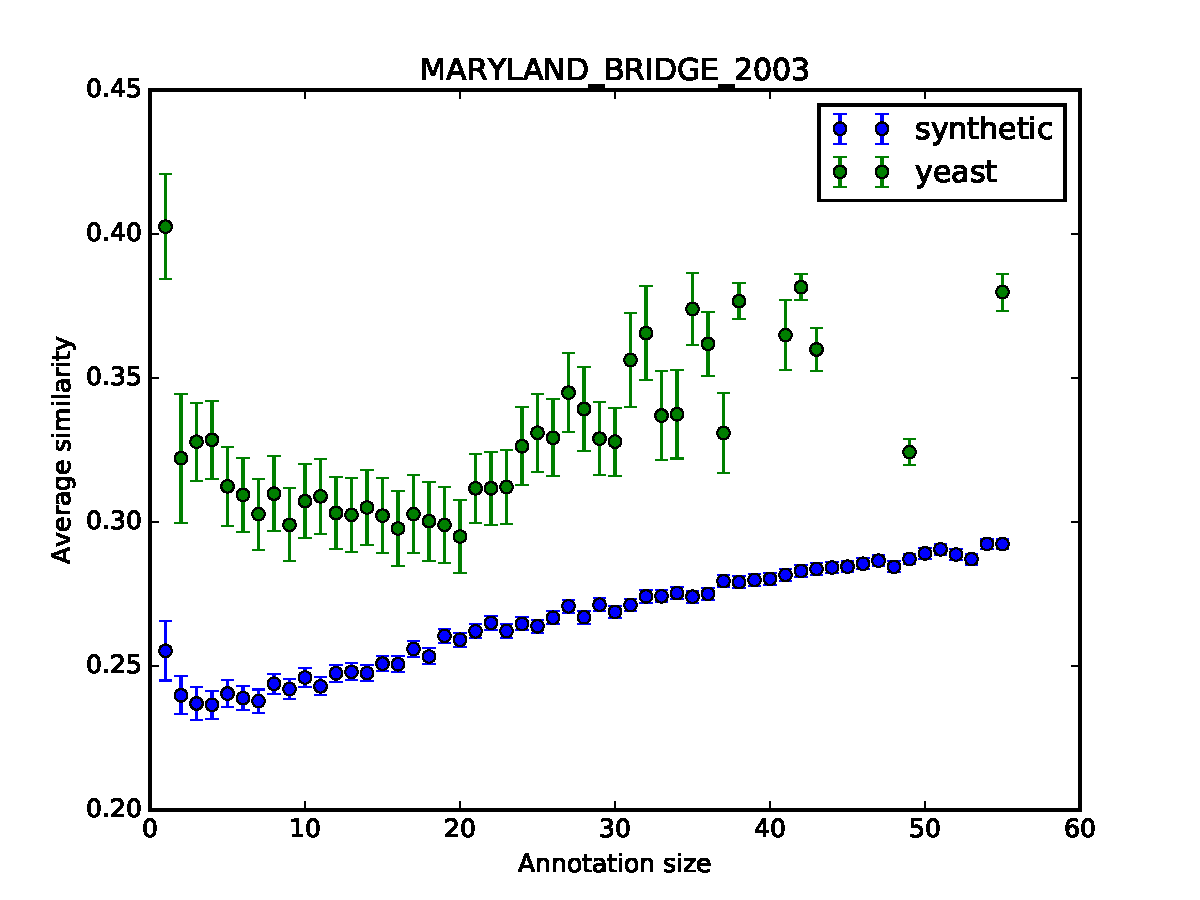
\includegraphics[width=0.5\linewidth, height=0.4\textheight]{groupwise/SIM_FRAMEWORK_DAG_SET_MARYLAND_BRIDGE_2003_avg.pdf}
\end{figure}

\end{frame}


%------------------------------------------------

\begin{frame}{Annotation size - Pairwise Similarity Measures}
\begin{figure}
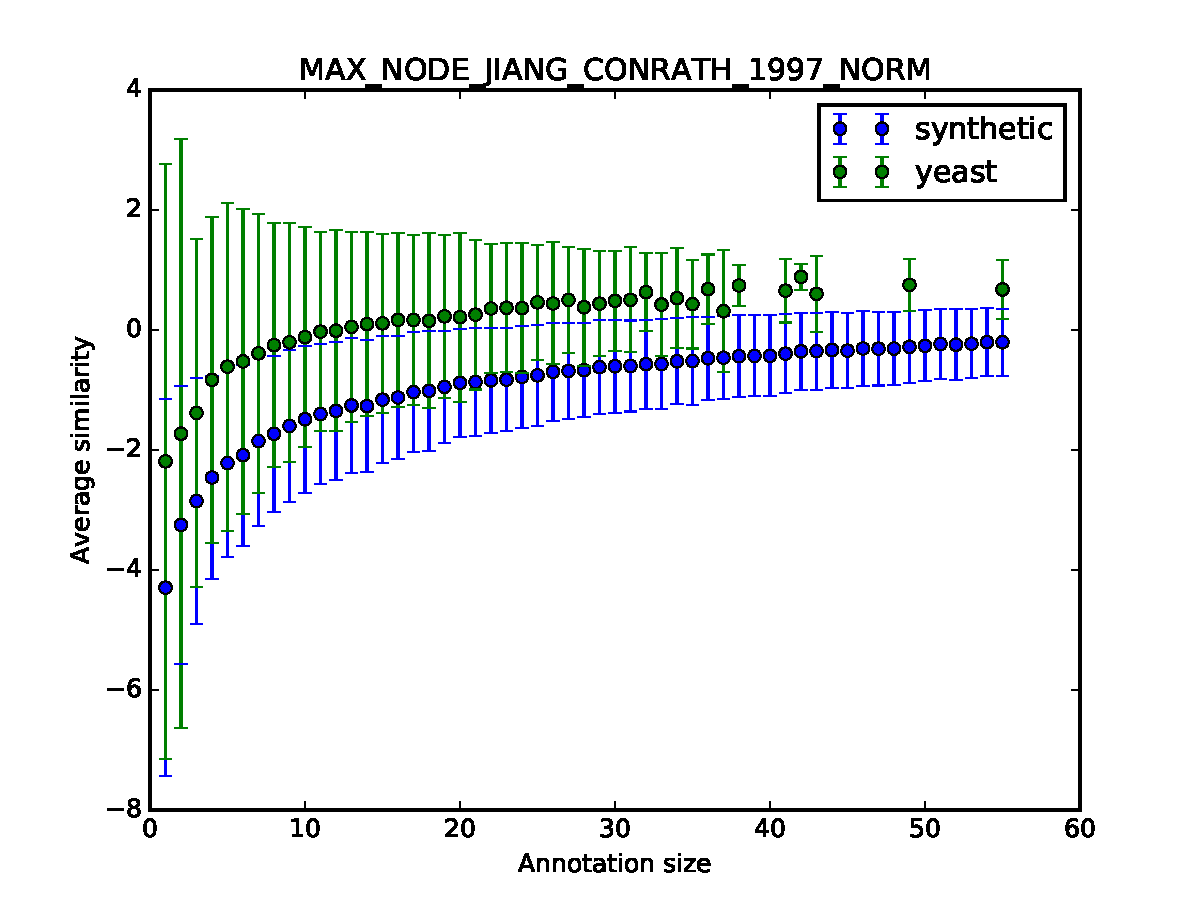
\includegraphics[width=0.5\linewidth, height=0.4\textheight]{pairwise/SIM_GROUPWISE_MAX_SIM_PAIRWISE_DAG_NODE_JIANG_CONRATH_1997_NORM_avg.pdf}
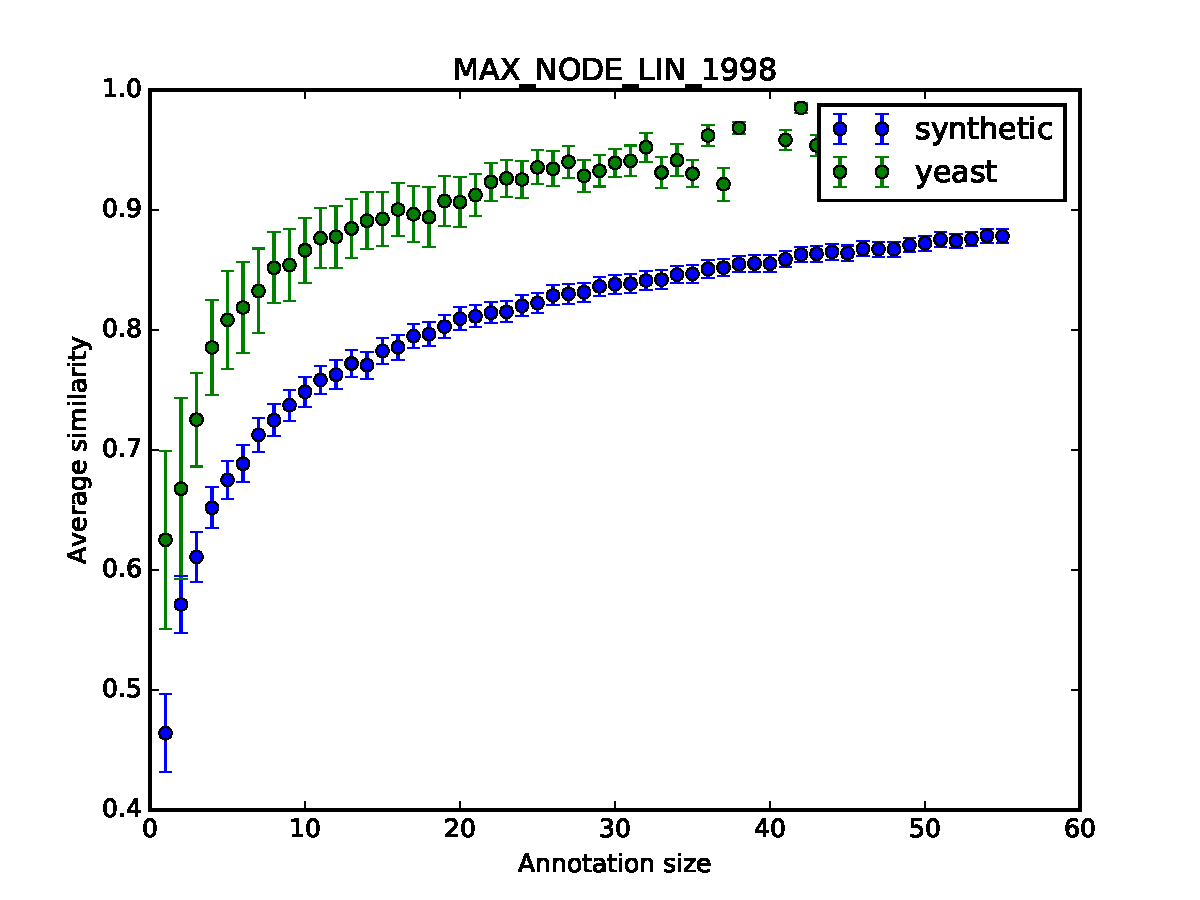
\includegraphics[width=0.5\linewidth, height=0.4\textheight]{pairwise/SIM_GROUPWISE_MAX_SIM_PAIRWISE_DAG_NODE_LIN_1998_avg.pdf} \\
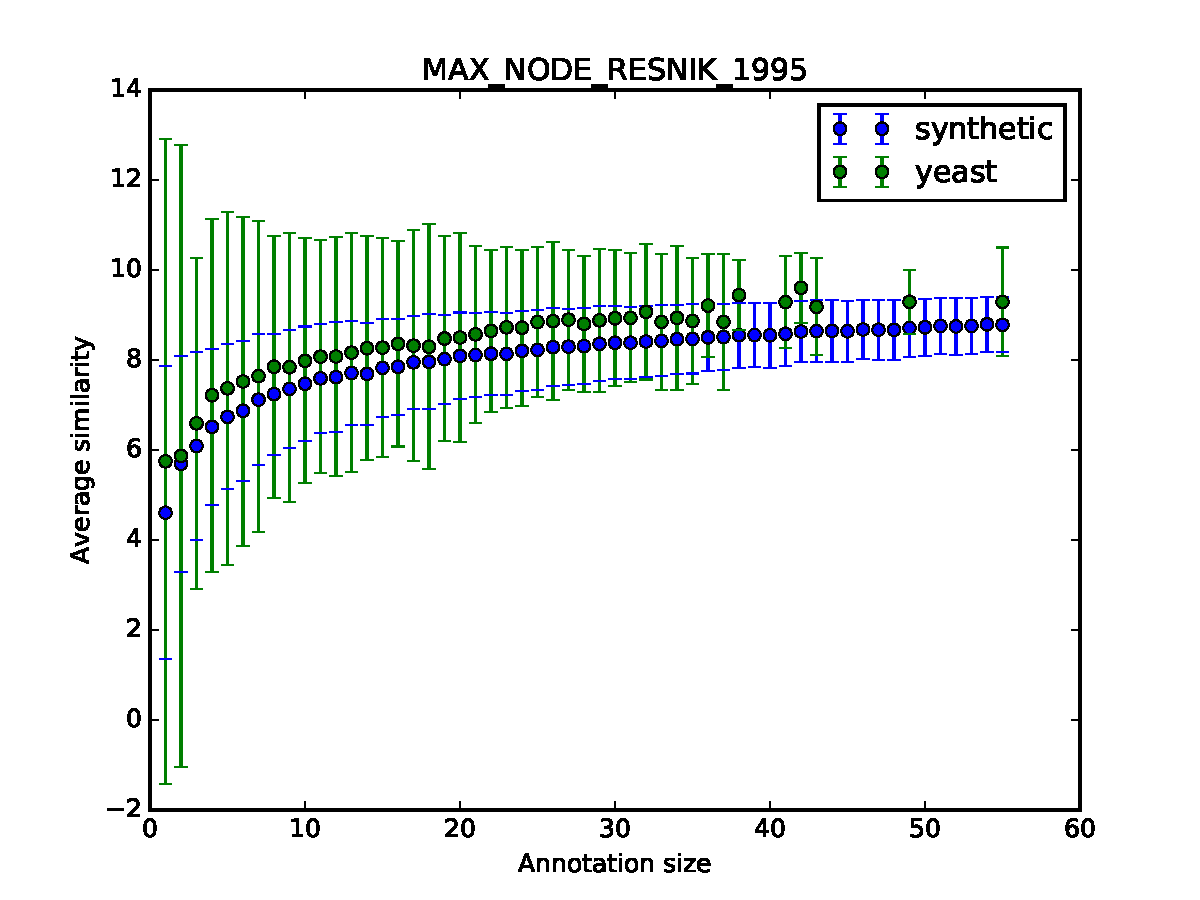
\includegraphics[width=0.5\linewidth, height=0.4\textheight]{pairwise/SIM_GROUPWISE_MAX_SIM_PAIRWISE_DAG_NODE_RESNIK_1995_avg.pdf}
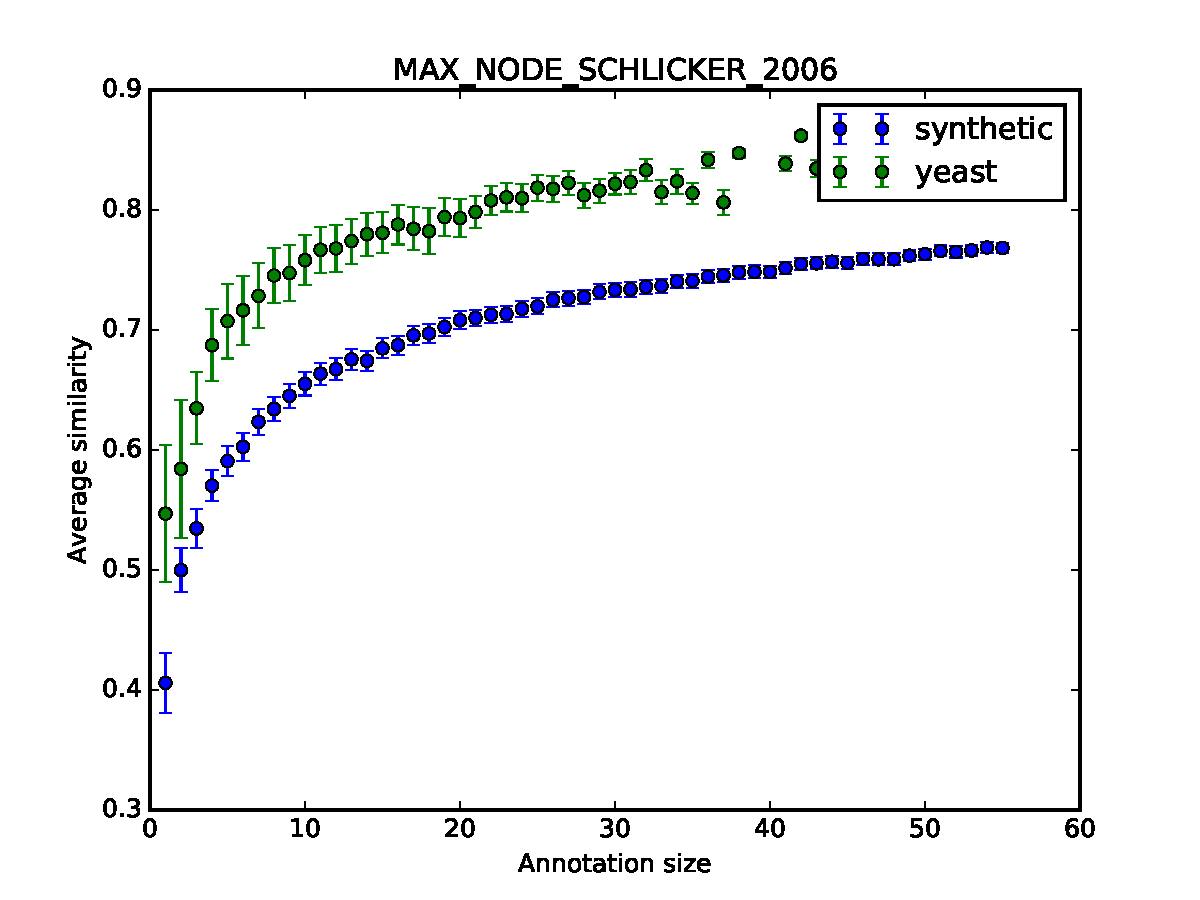
\includegraphics[width=0.5\linewidth, height=0.4\textheight]{pairwise/SIM_GROUPWISE_MAX_SIM_PAIRWISE_DAG_NODE_SCHLICKER_2006_avg.pdf}
\end{figure}
\end{frame}

\begin{frame}{Annotation size - Pairwise Similarity Measures}
\begin{figure}
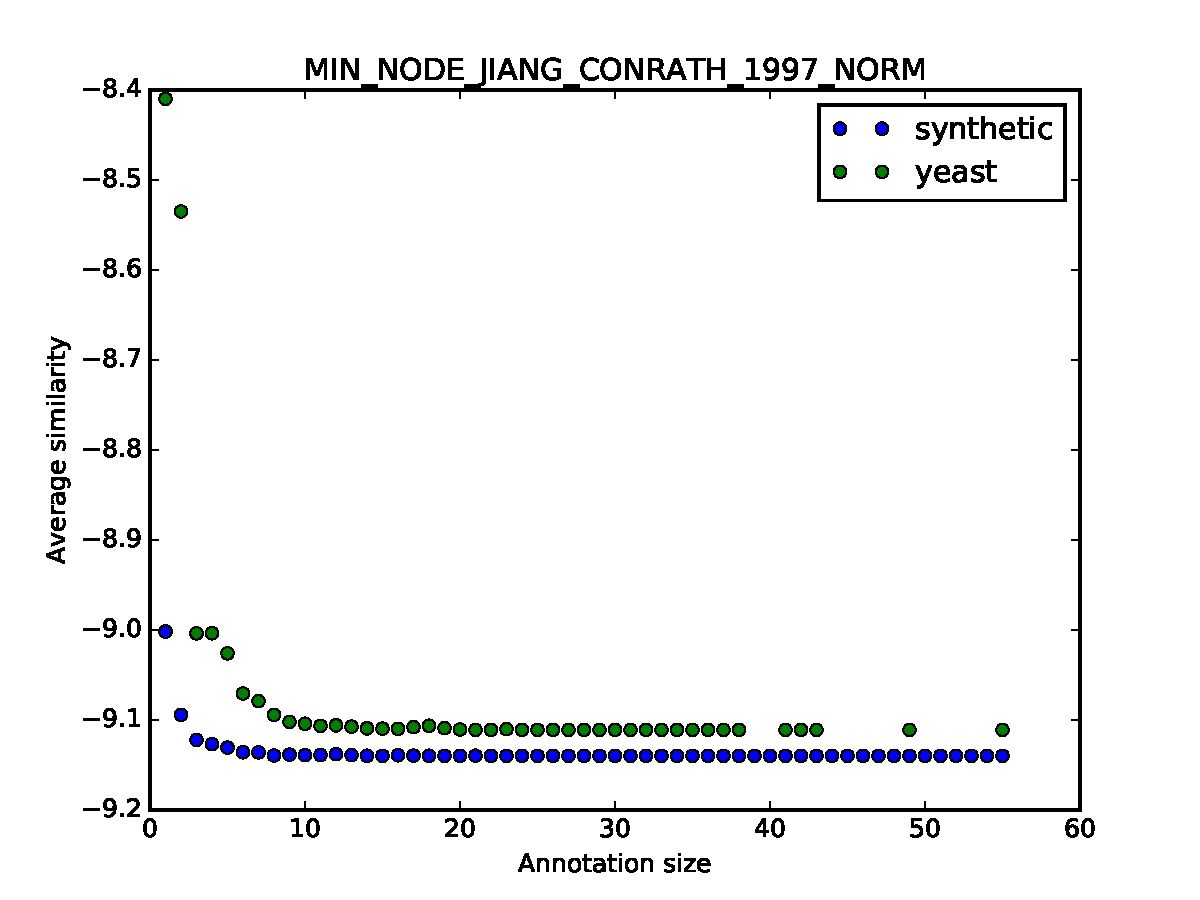
\includegraphics[width=0.5\linewidth, height=0.4\textheight]{pairwise/SIM_GROUPWISE_MIN_SIM_PAIRWISE_DAG_NODE_JIANG_CONRATH_1997_NORM_avg.pdf}
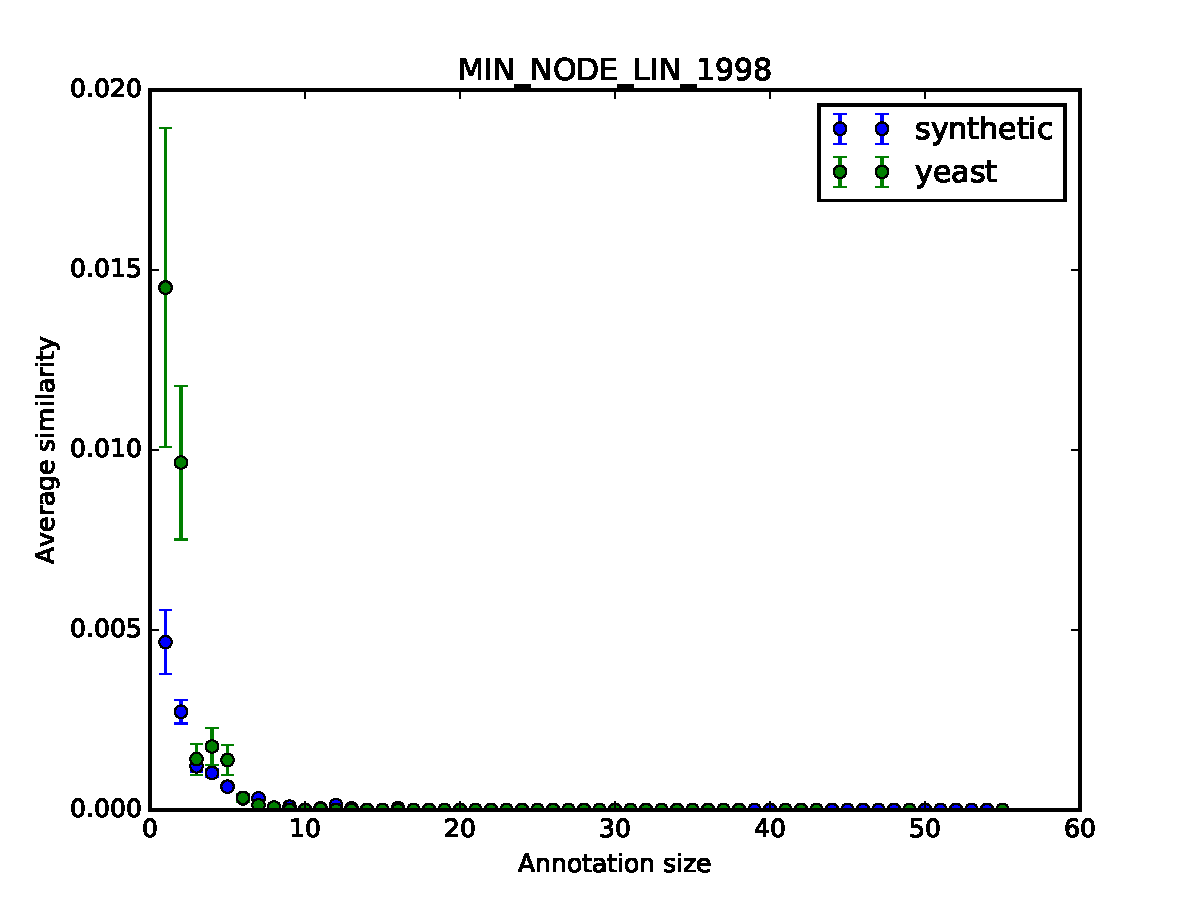
\includegraphics[width=0.5\linewidth, height=0.4\textheight]{pairwise/SIM_GROUPWISE_MIN_SIM_PAIRWISE_DAG_NODE_LIN_1998_avg.pdf} \\
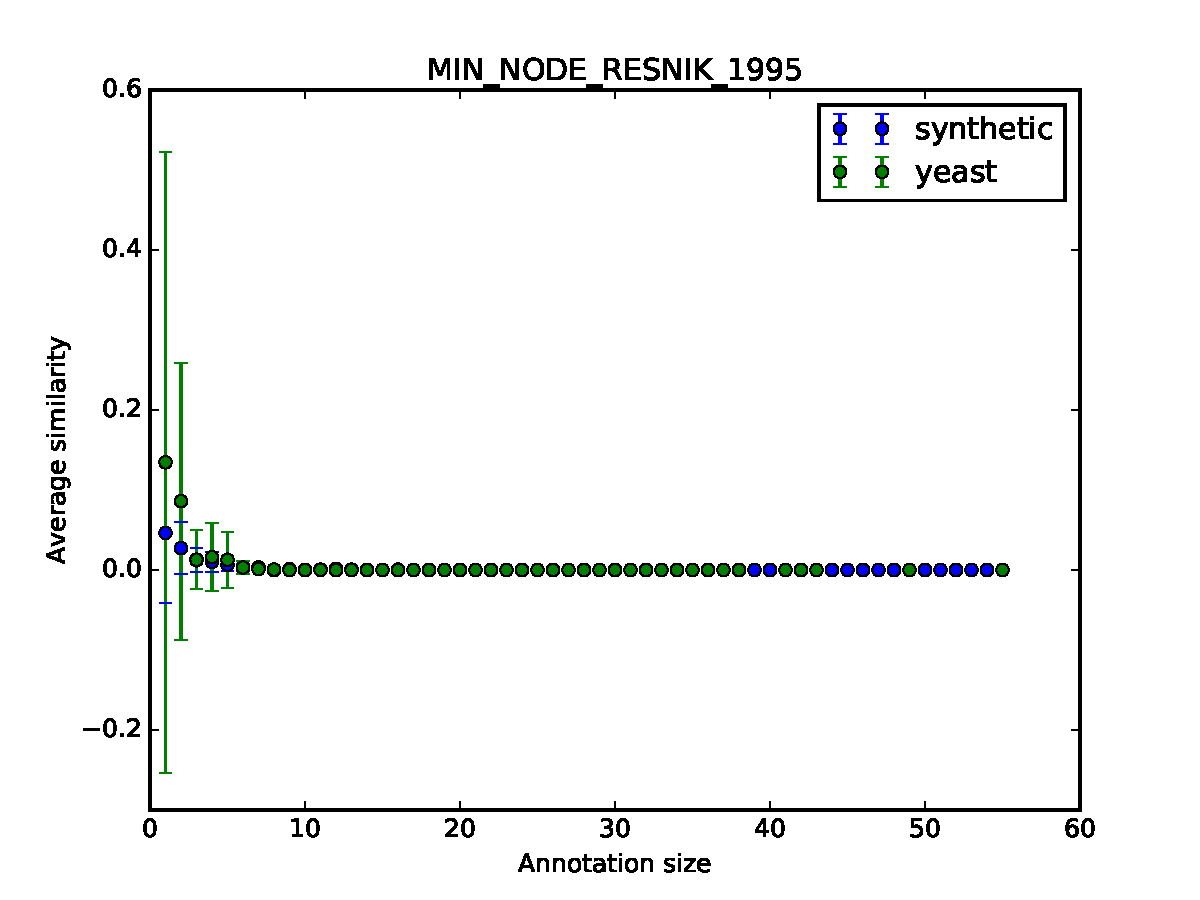
\includegraphics[width=0.5\linewidth, height=0.4\textheight]{pairwise/SIM_GROUPWISE_MIN_SIM_PAIRWISE_DAG_NODE_RESNIK_1995_avg.pdf}
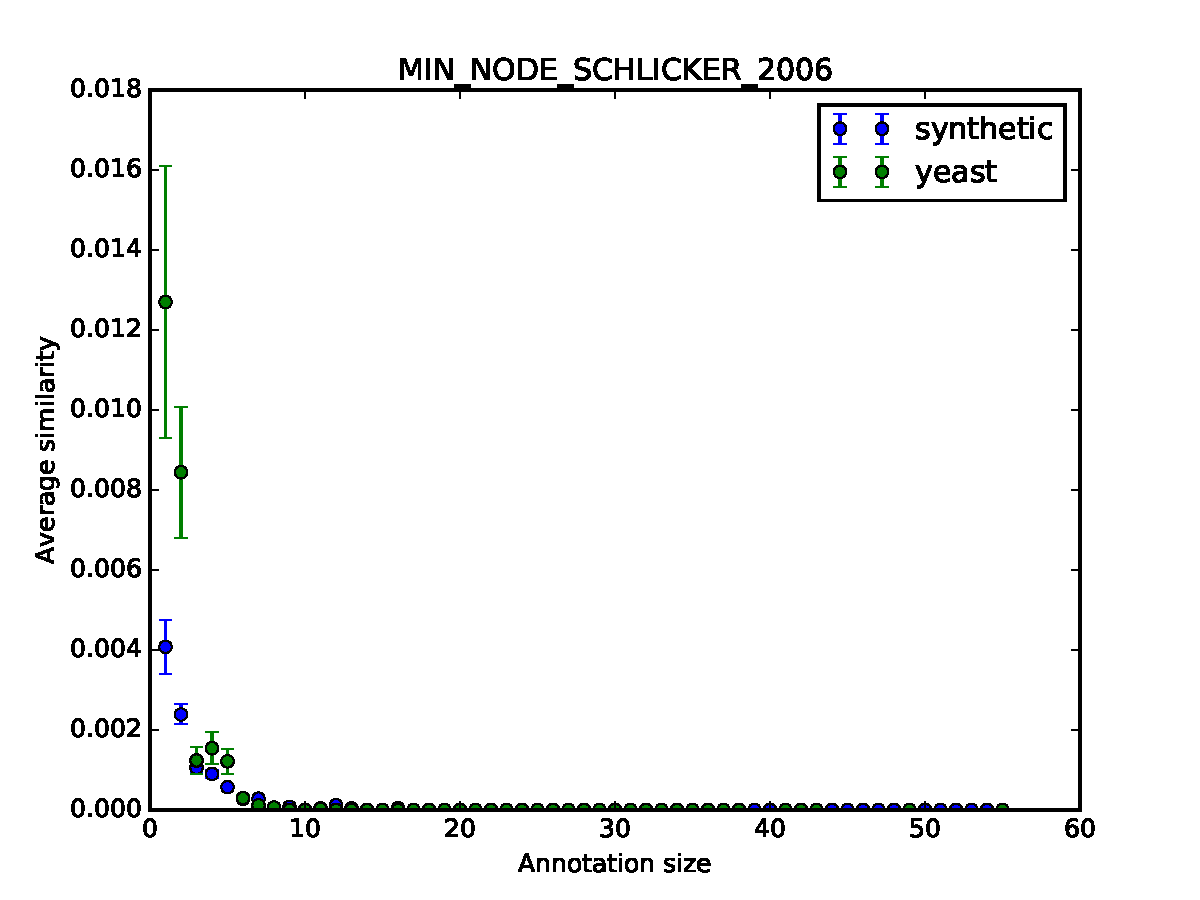
\includegraphics[width=0.5\linewidth, height=0.4\textheight]{pairwise/SIM_GROUPWISE_MIN_SIM_PAIRWISE_DAG_NODE_SCHLICKER_2006_avg.pdf}
\end{figure}
\end{frame}


\begin{frame}{Annotation size - Pairwise Similarity Measures}

\begin{figure}

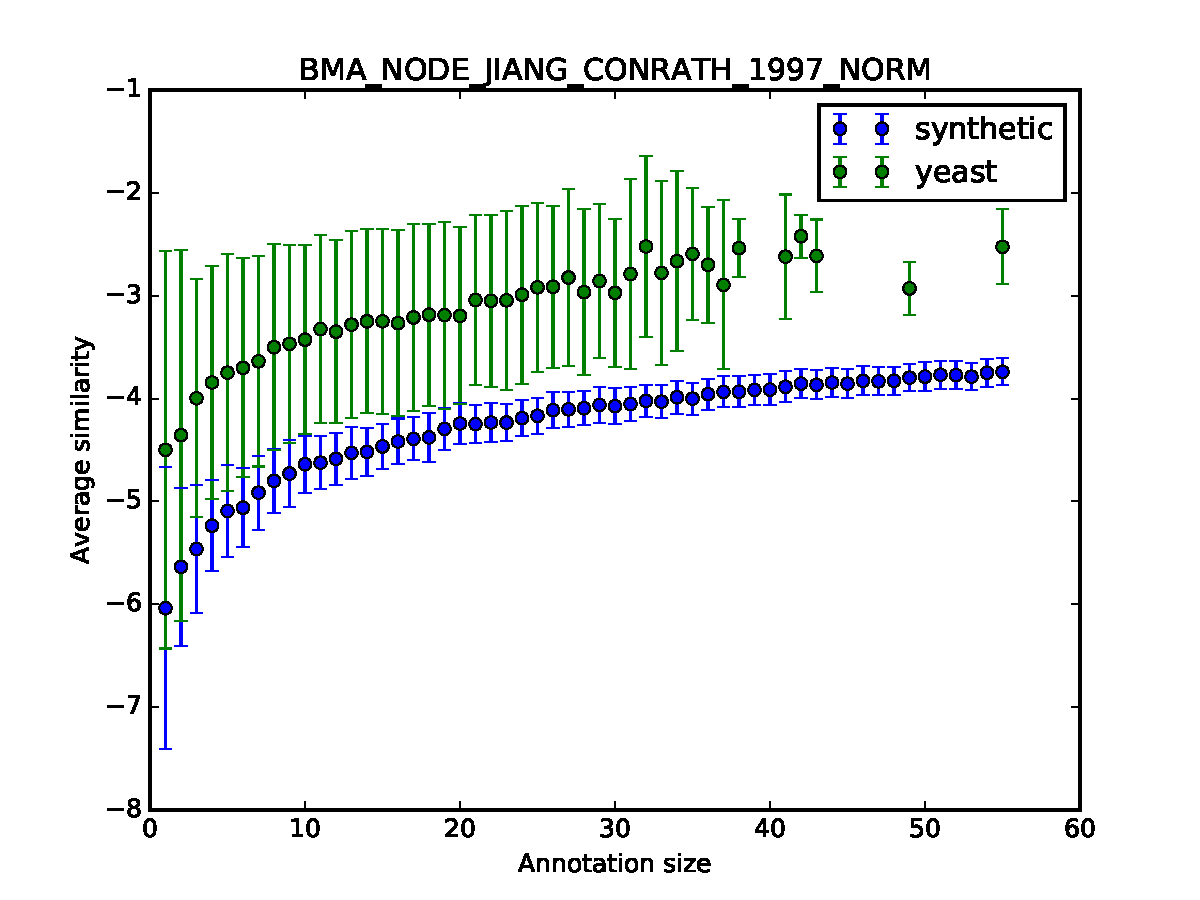
\includegraphics[width=0.5\linewidth, height=0.4\textheight]{pairwise/SIM_GROUPWISE_BMA_SIM_PAIRWISE_DAG_NODE_JIANG_CONRATH_1997_NORM_avg.pdf}
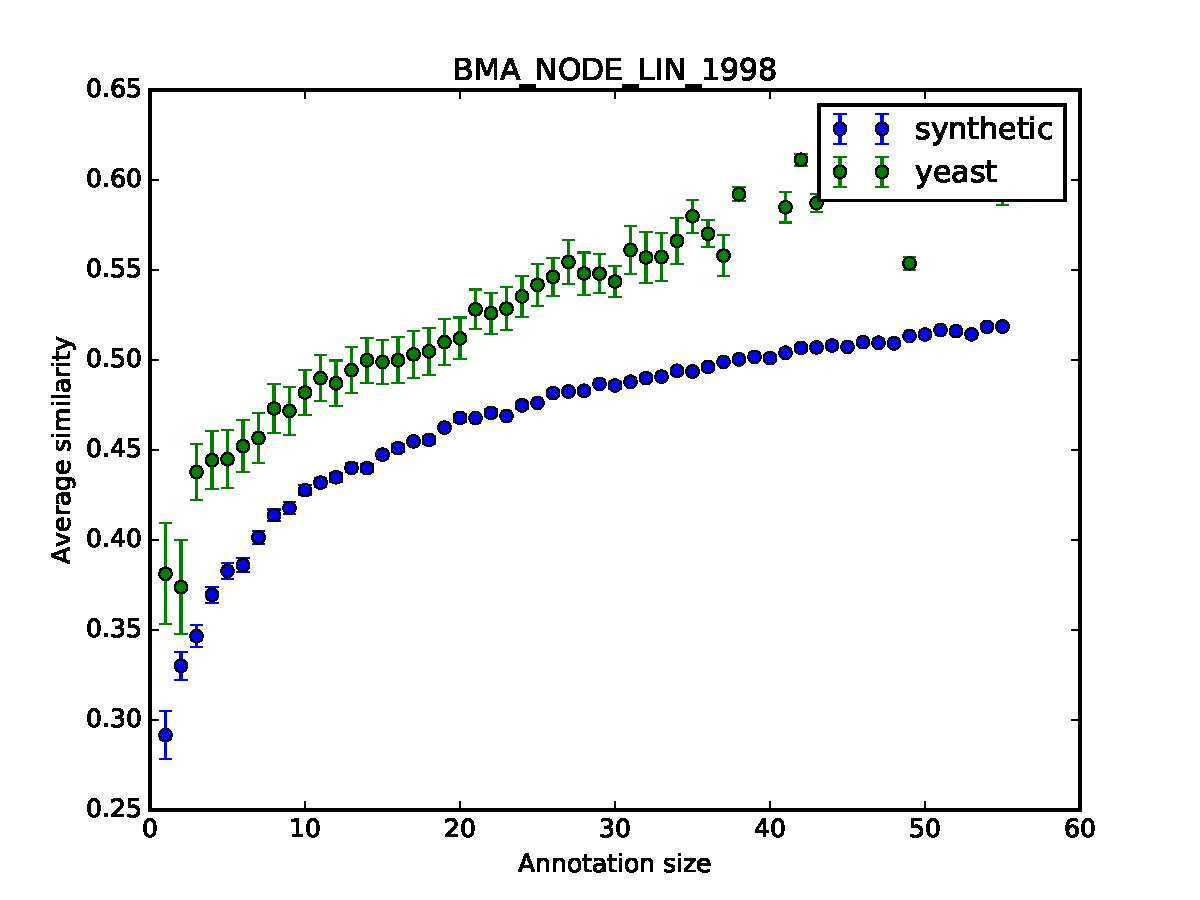
\includegraphics[width=0.5\linewidth, height=0.4\textheight]{pairwise/SIM_GROUPWISE_BMA_SIM_PAIRWISE_DAG_NODE_LIN_1998_avg.pdf}\\
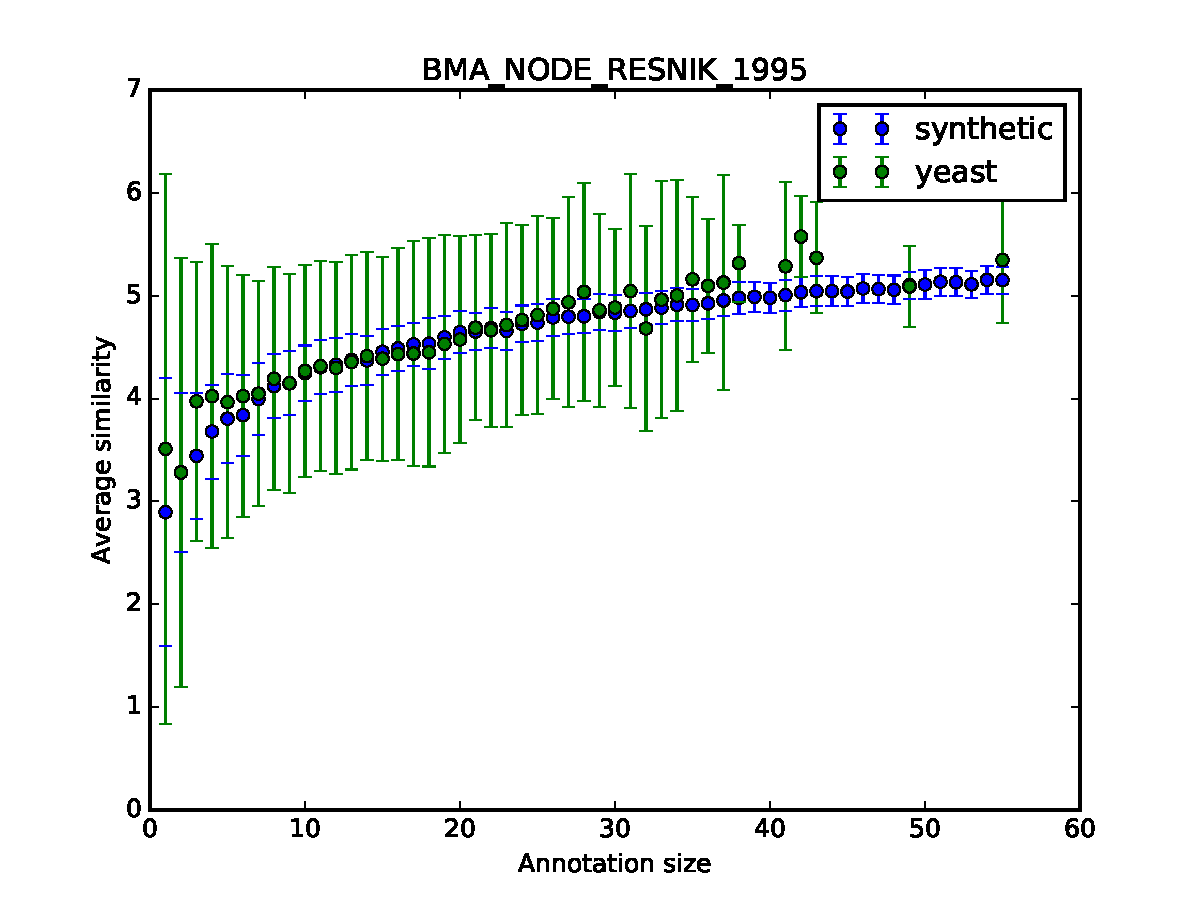
\includegraphics[width=0.5\linewidth, height=0.4\textheight]{pairwise/SIM_GROUPWISE_BMA_SIM_PAIRWISE_DAG_NODE_RESNIK_1995_avg.pdf}
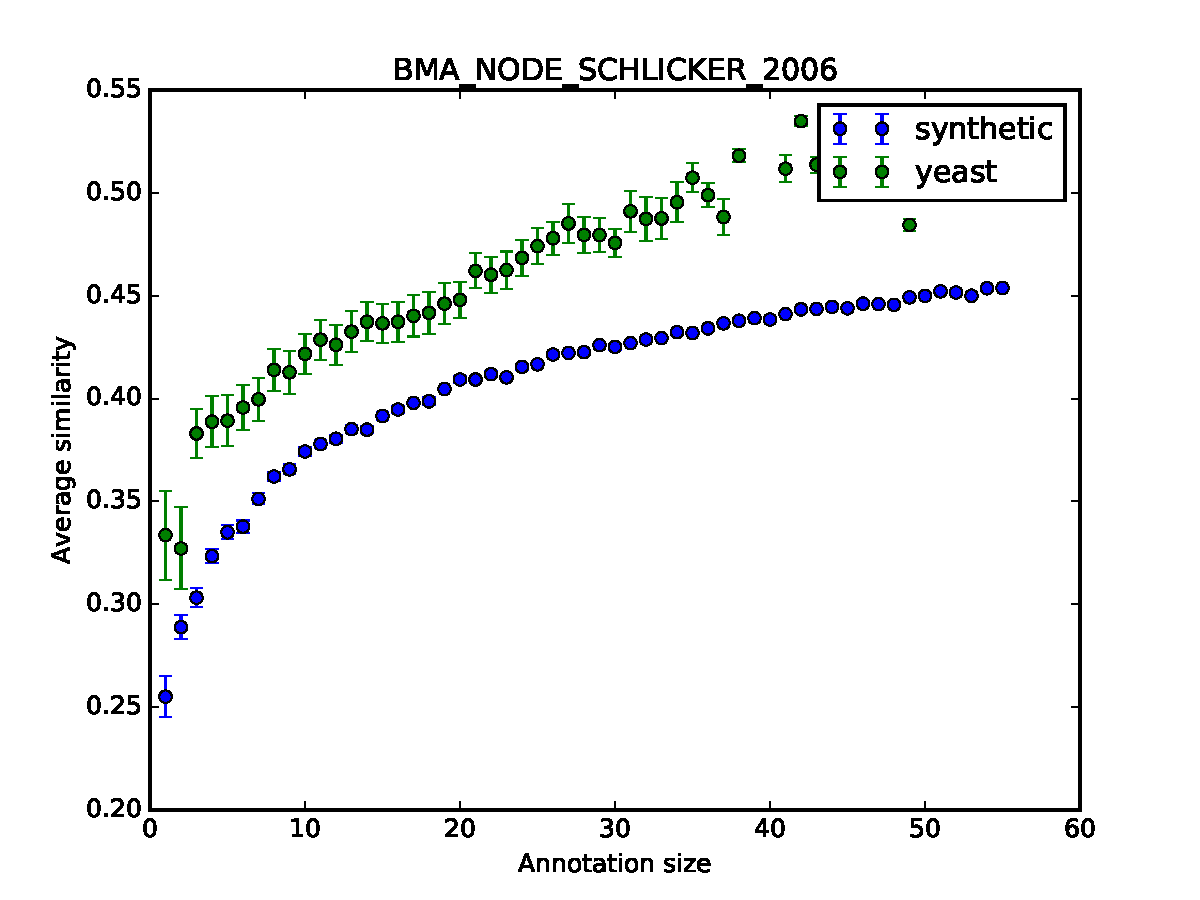
\includegraphics[width=0.5\linewidth, height=0.4\textheight]{pairwise/SIM_GROUPWISE_BMA_SIM_PAIRWISE_DAG_NODE_SCHLICKER_2006_avg.pdf}
\end{figure}

\end{frame}

\begin{frame}{Annotation size - Pairwise Similarity Measures}

\begin{figure}
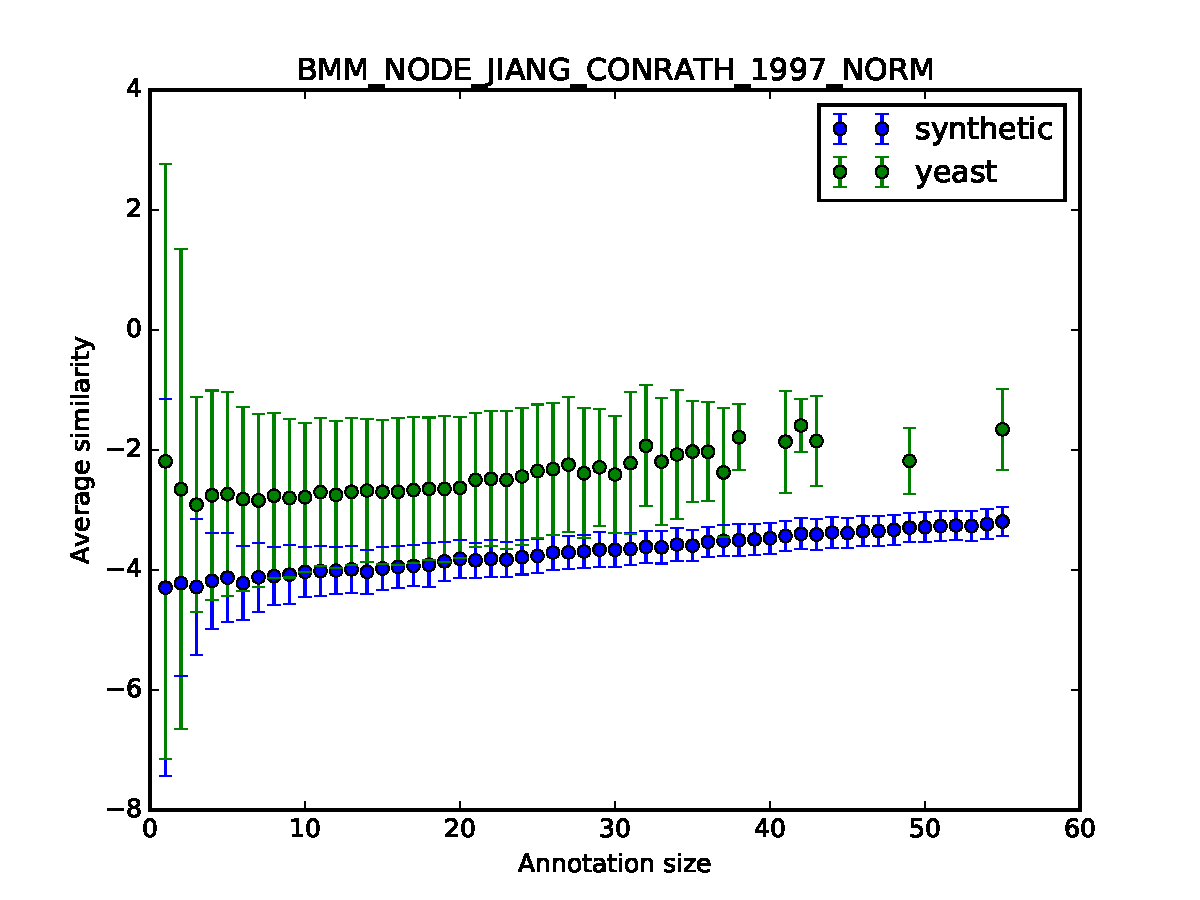
\includegraphics[width=0.5\linewidth, height=0.4\textheight]{pairwise/SIM_GROUPWISE_BMM_SIM_PAIRWISE_DAG_NODE_JIANG_CONRATH_1997_NORM_avg.pdf} 
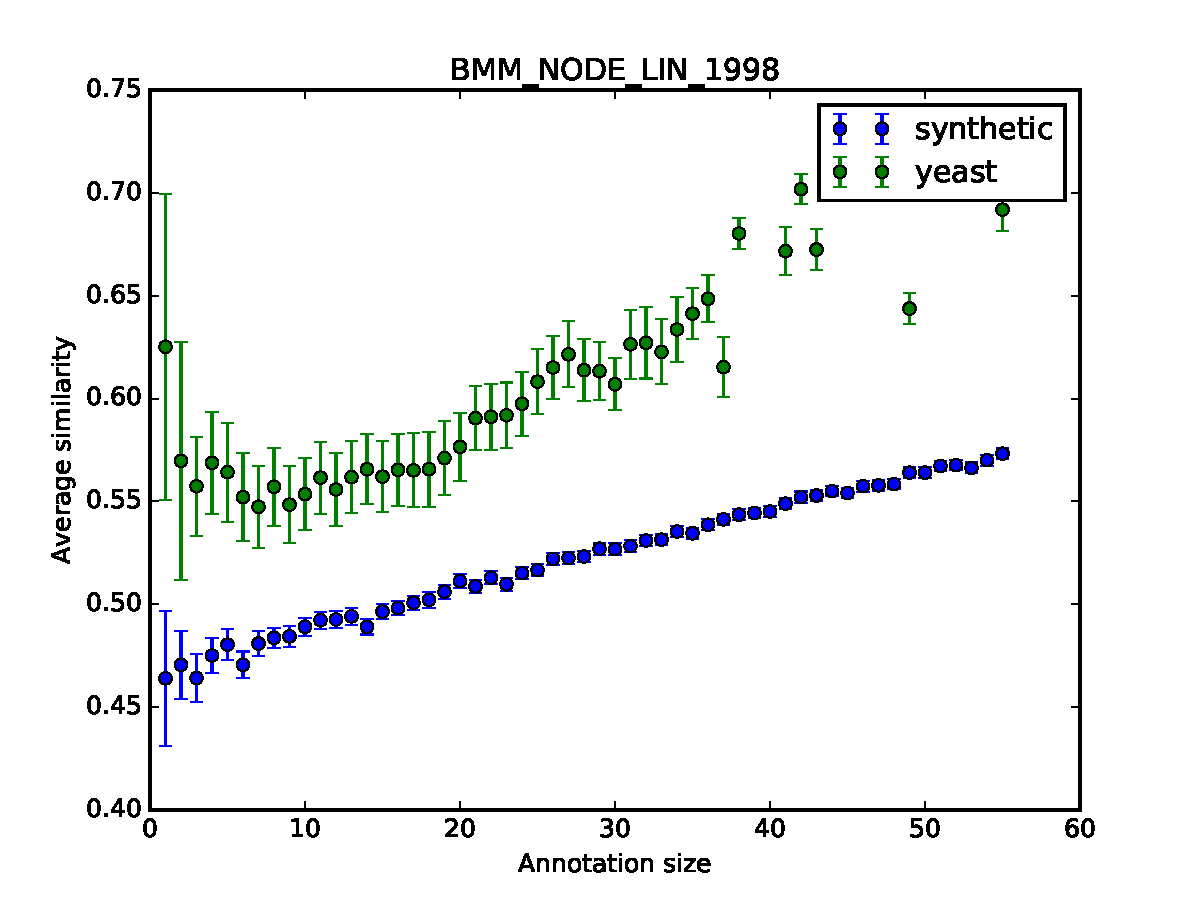
\includegraphics[width=0.5\linewidth, height=0.4\textheight]{pairwise/SIM_GROUPWISE_BMM_SIM_PAIRWISE_DAG_NODE_LIN_1998_avg.pdf}\\
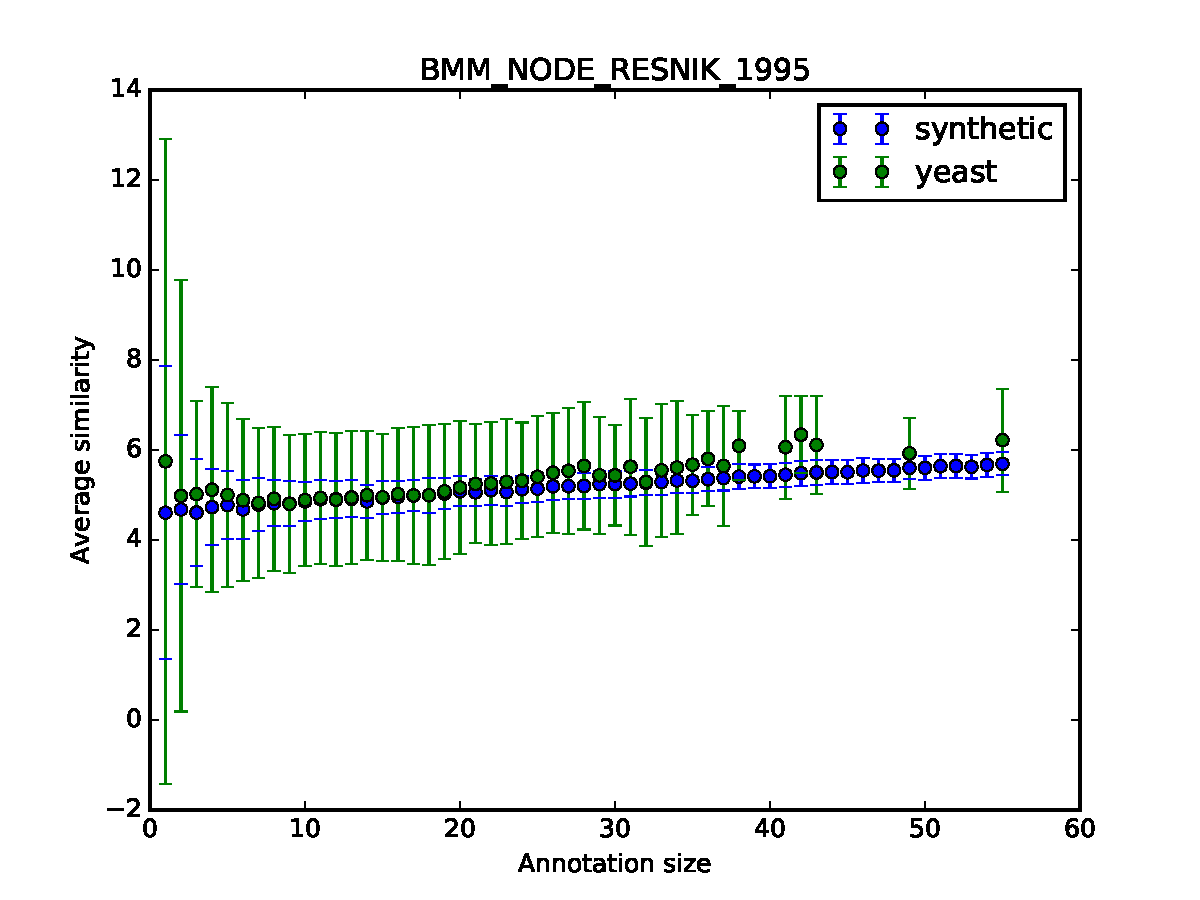
\includegraphics[width=0.5\linewidth, height=0.4\textheight]{pairwise/SIM_GROUPWISE_BMM_SIM_PAIRWISE_DAG_NODE_RESNIK_1995_avg.pdf}
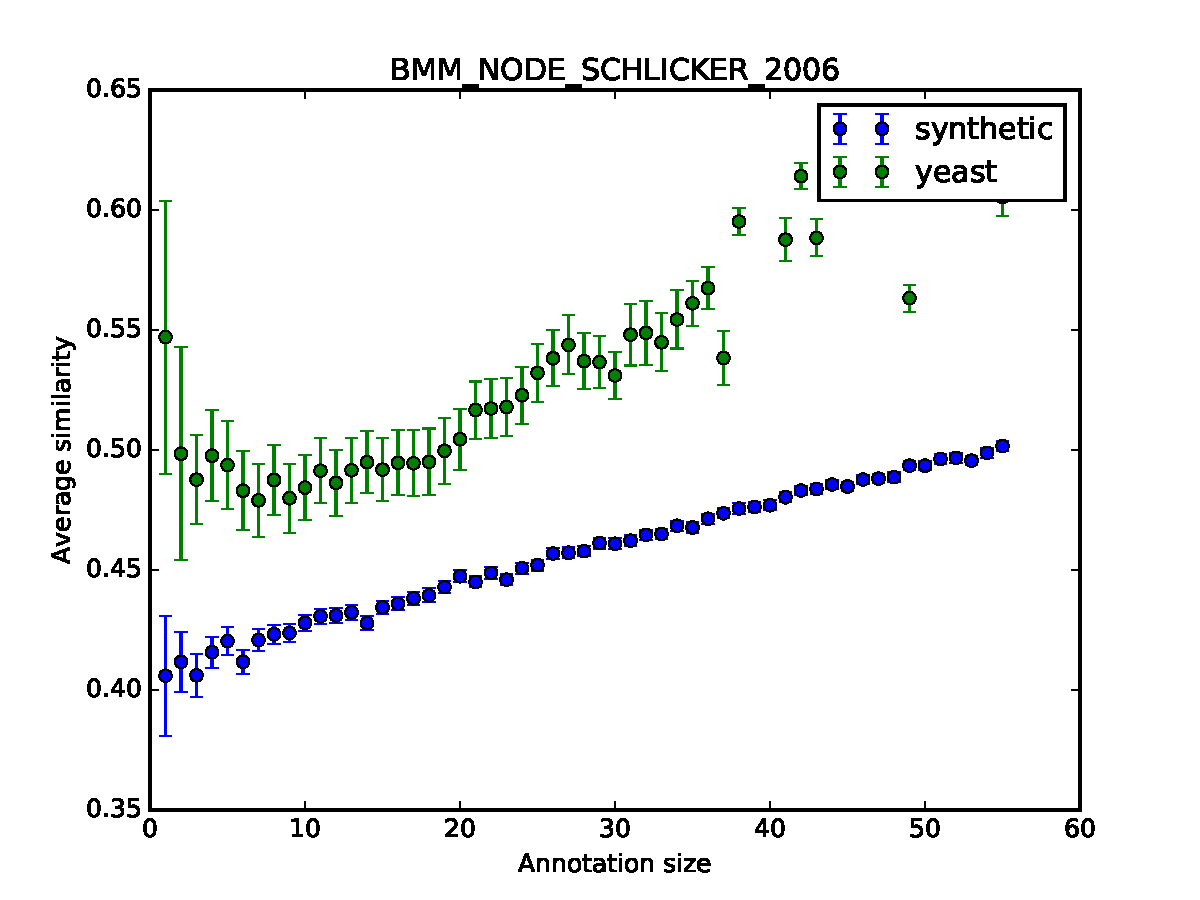
\includegraphics[width=0.5\linewidth, height=0.4\textheight]{pairwise/SIM_GROUPWISE_BMM_SIM_PAIRWISE_DAG_NODE_SCHLICKER_2006_avg.pdf}
\end{figure}

\end{frame}

\begin{frame}{Annotation size - Pairwise Similarity Measures}

\begin{figure}
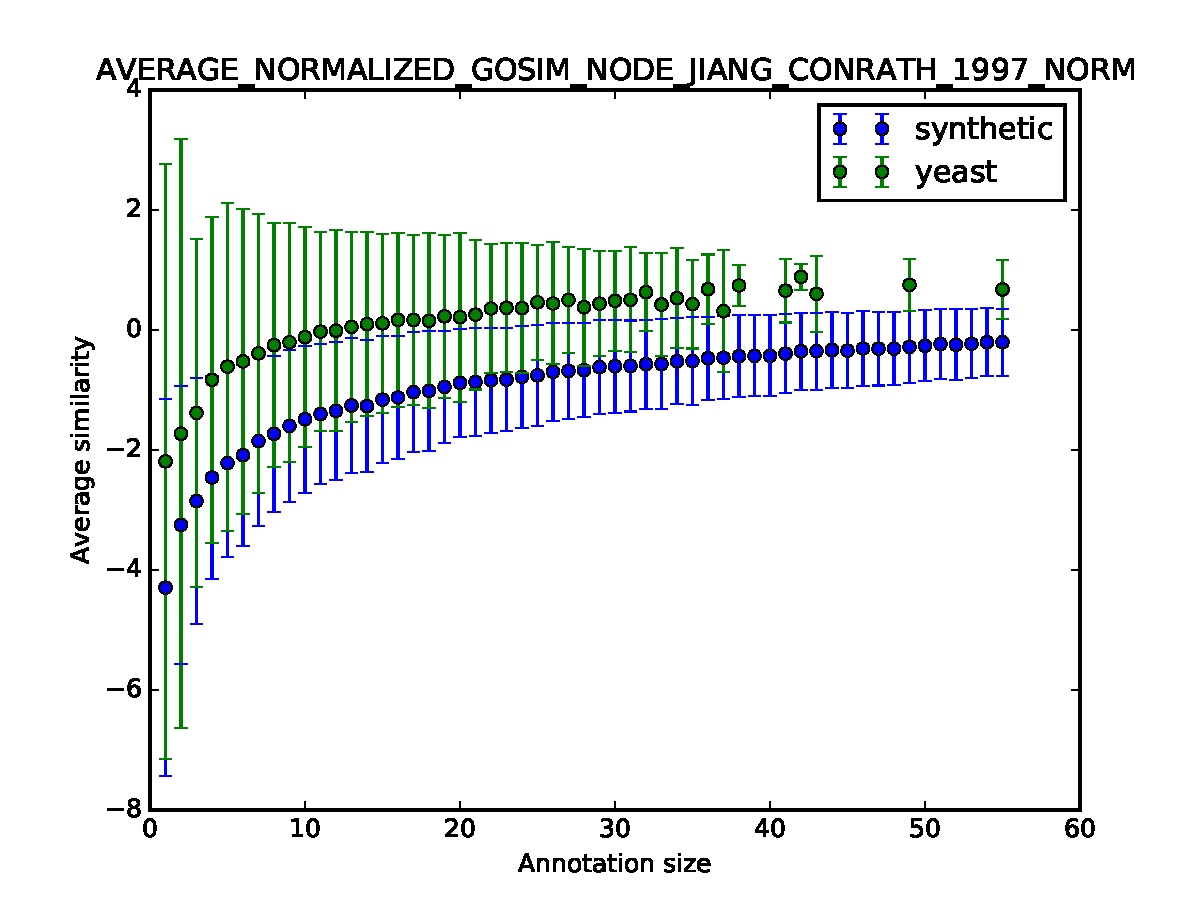
\includegraphics[width=0.5\linewidth, height=0.4\textheight]{pairwise/SIM_GROUPWISE_AVERAGE_NORMALIZED_GOSIM_SIM_PAIRWISE_DAG_NODE_JIANG_CONRATH_1997_NORM_avg.pdf}
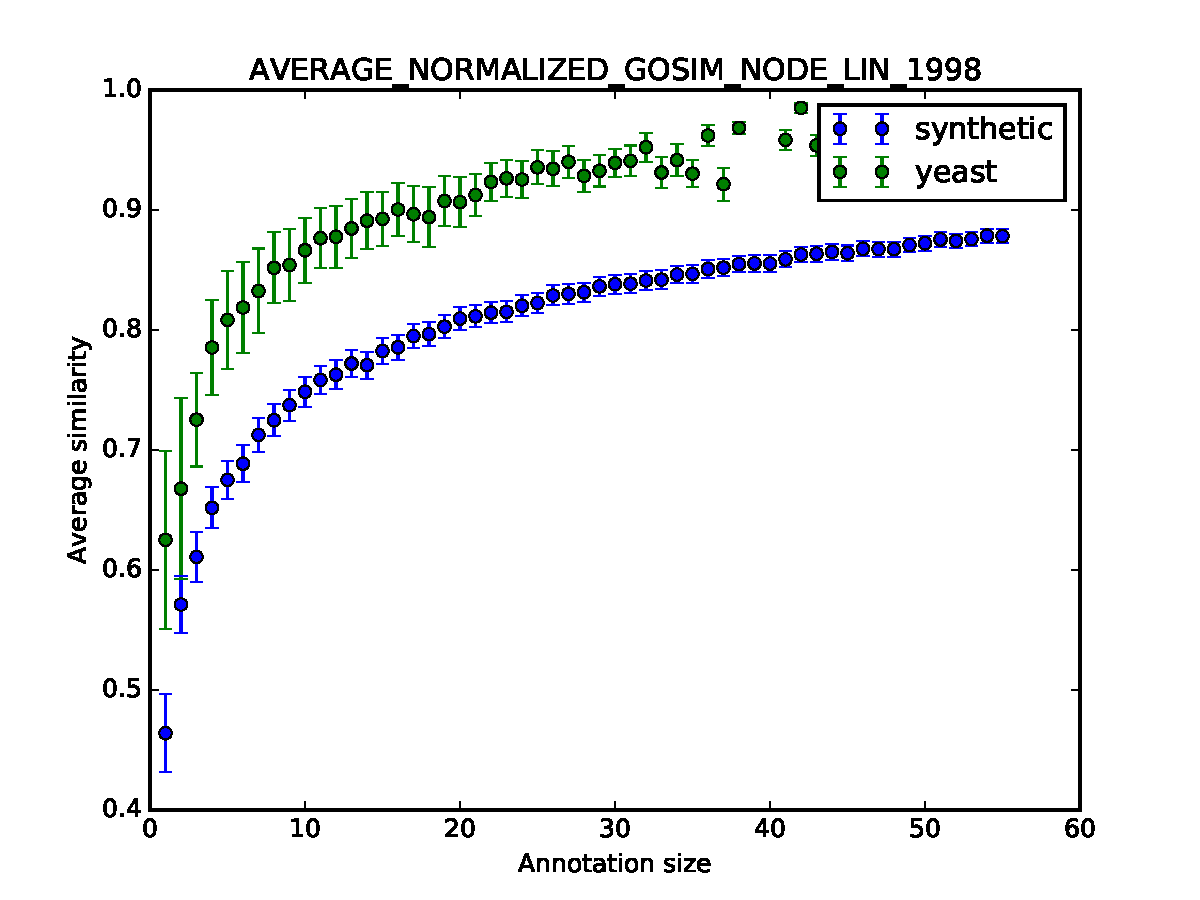
\includegraphics[width=0.5\linewidth, height=0.4\textheight]{pairwise/SIM_GROUPWISE_AVERAGE_NORMALIZED_GOSIM_SIM_PAIRWISE_DAG_NODE_LIN_1998_avg.pdf} \\
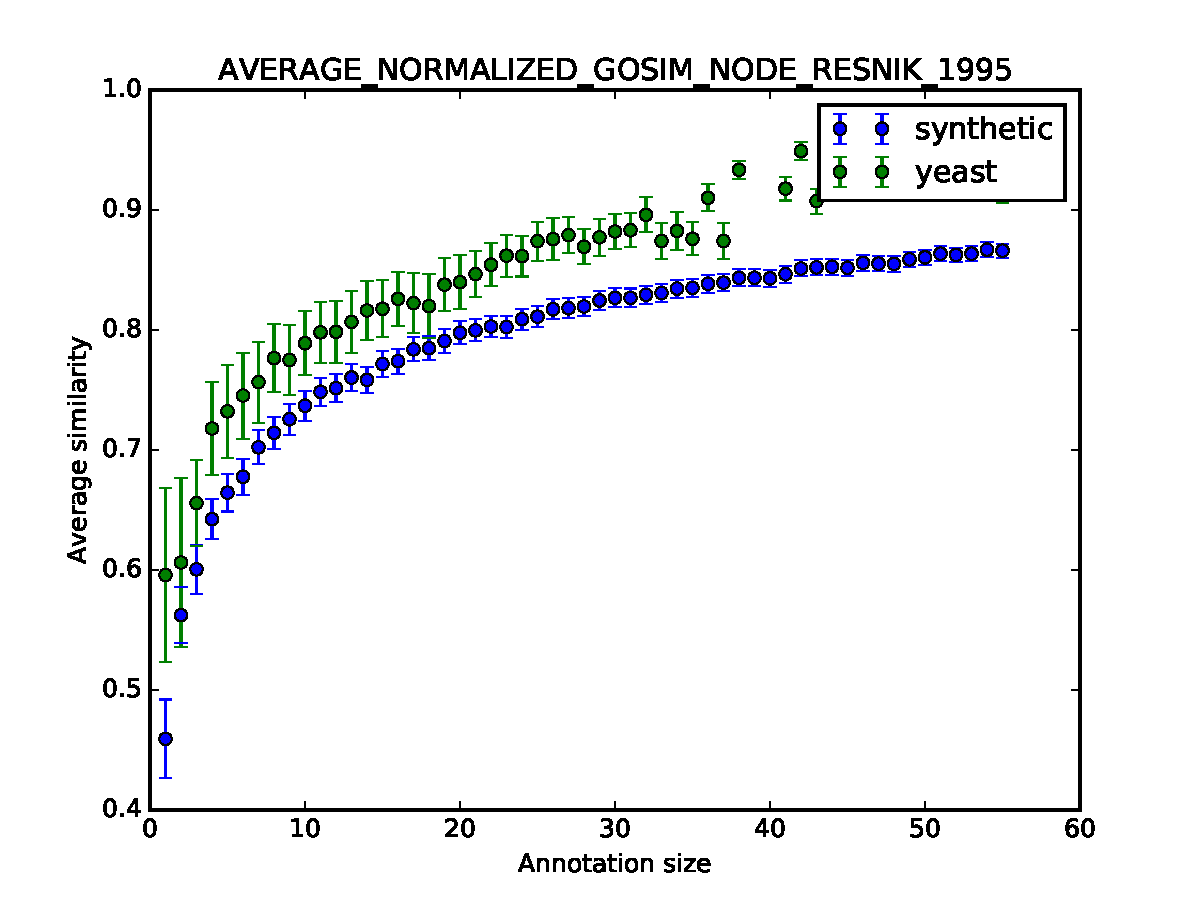
\includegraphics[width=0.5\linewidth, height=0.4\textheight]{pairwise/SIM_GROUPWISE_AVERAGE_NORMALIZED_GOSIM_SIM_PAIRWISE_DAG_NODE_RESNIK_1995_avg.pdf}
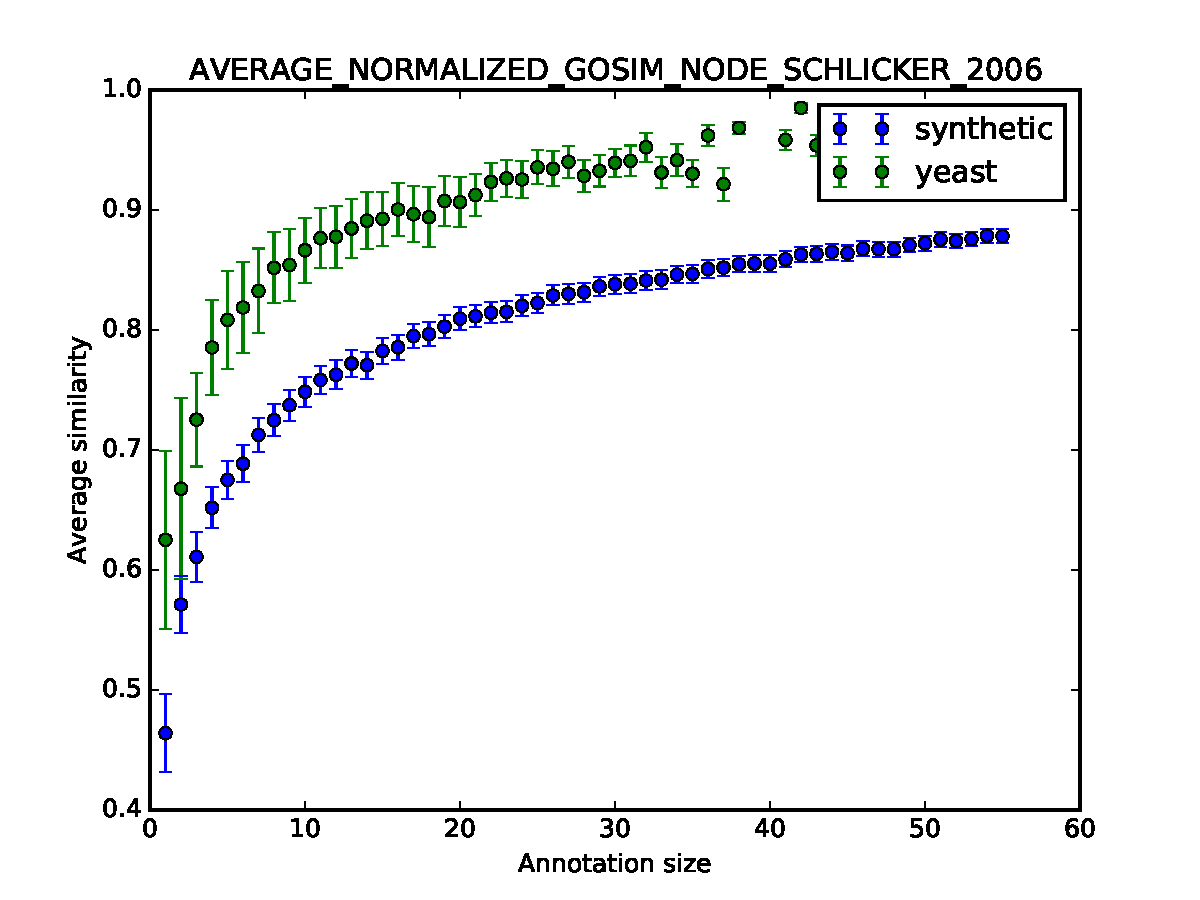
\includegraphics[width=0.5\linewidth, height=0.4\textheight]{pairwise/SIM_GROUPWISE_AVERAGE_NORMALIZED_GOSIM_SIM_PAIRWISE_DAG_NODE_SCHLICKER_2006_avg.pdf}
\end{figure}

\end{frame}



\begin{frame}{Annotation size - Pairwise Similarity Measures}

\begin{figure}
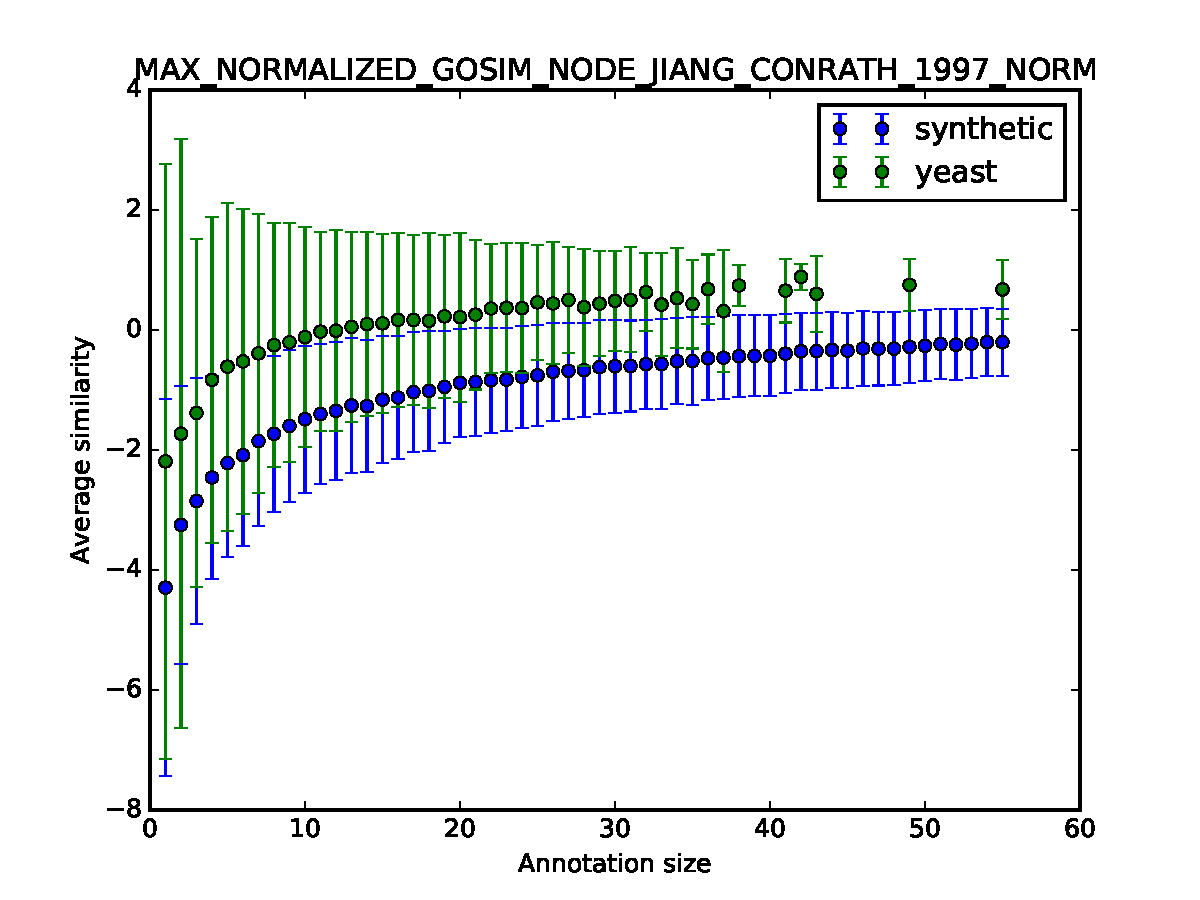
\includegraphics[width=0.5\linewidth, height=0.4\textheight]{pairwise/SIM_GROUPWISE_MAX_NORMALIZED_GOSIM_SIM_PAIRWISE_DAG_NODE_JIANG_CONRATH_1997_NORM_avg.pdf}
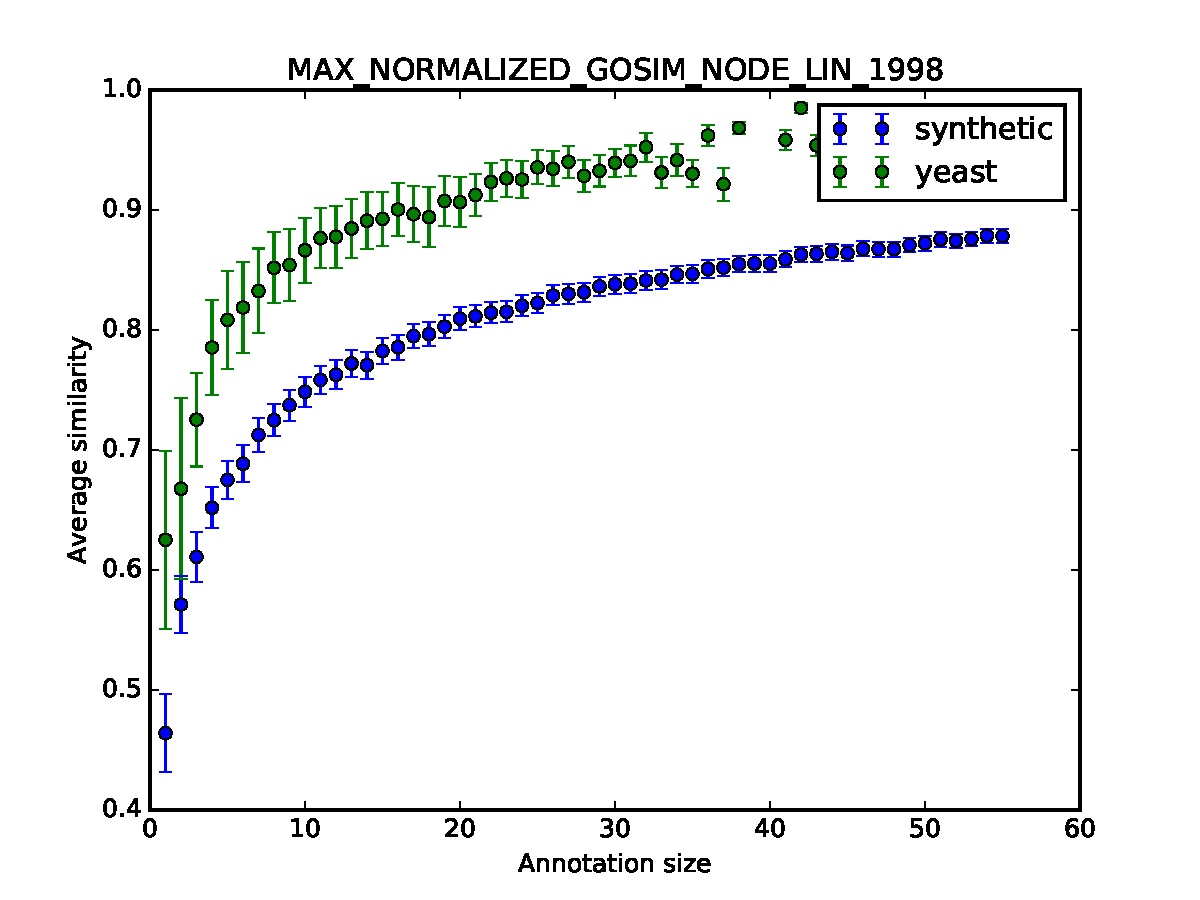
\includegraphics[width=0.5\linewidth, height=0.4\textheight]{pairwise/SIM_GROUPWISE_MAX_NORMALIZED_GOSIM_SIM_PAIRWISE_DAG_NODE_LIN_1998_avg.pdf} \\
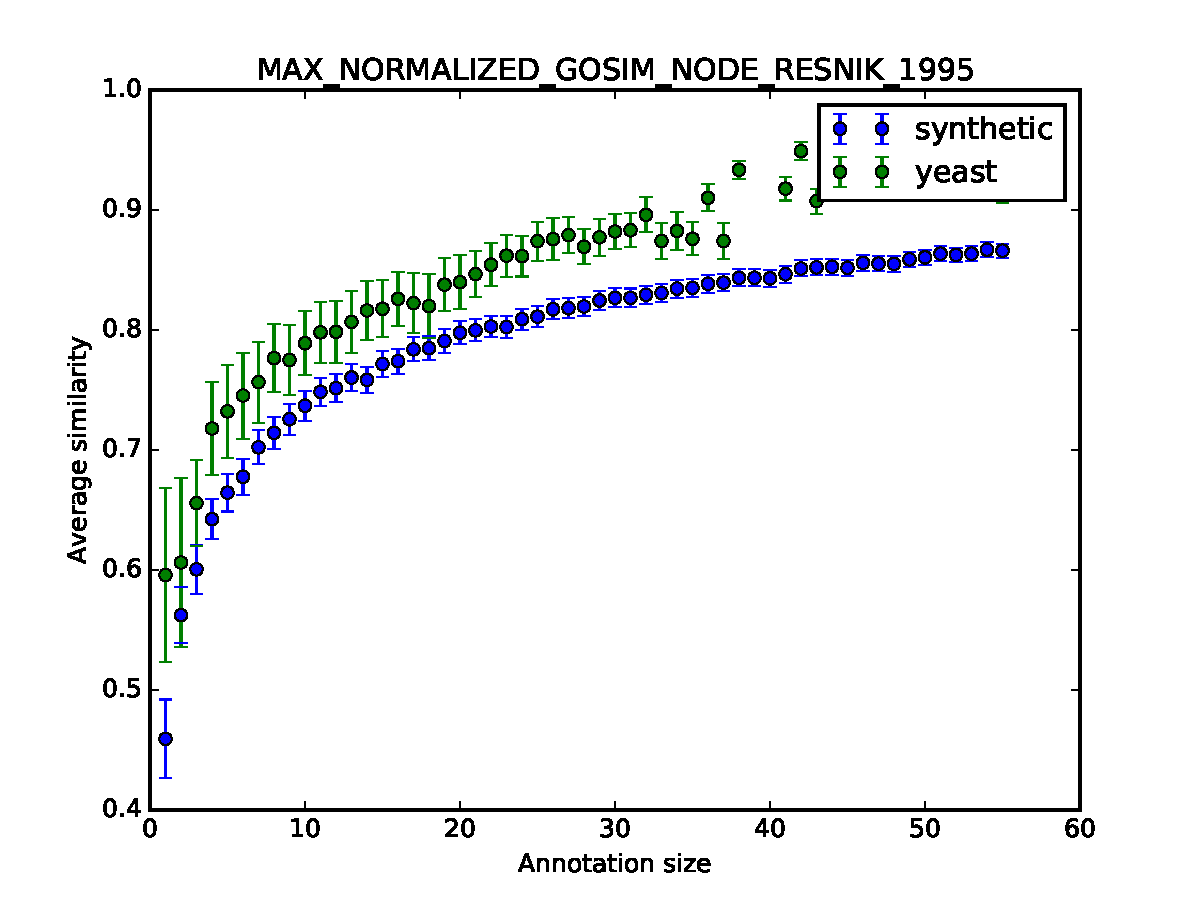
\includegraphics[width=0.5\linewidth, height=0.4\textheight]{pairwise/SIM_GROUPWISE_MAX_NORMALIZED_GOSIM_SIM_PAIRWISE_DAG_NODE_RESNIK_1995_avg.pdf}
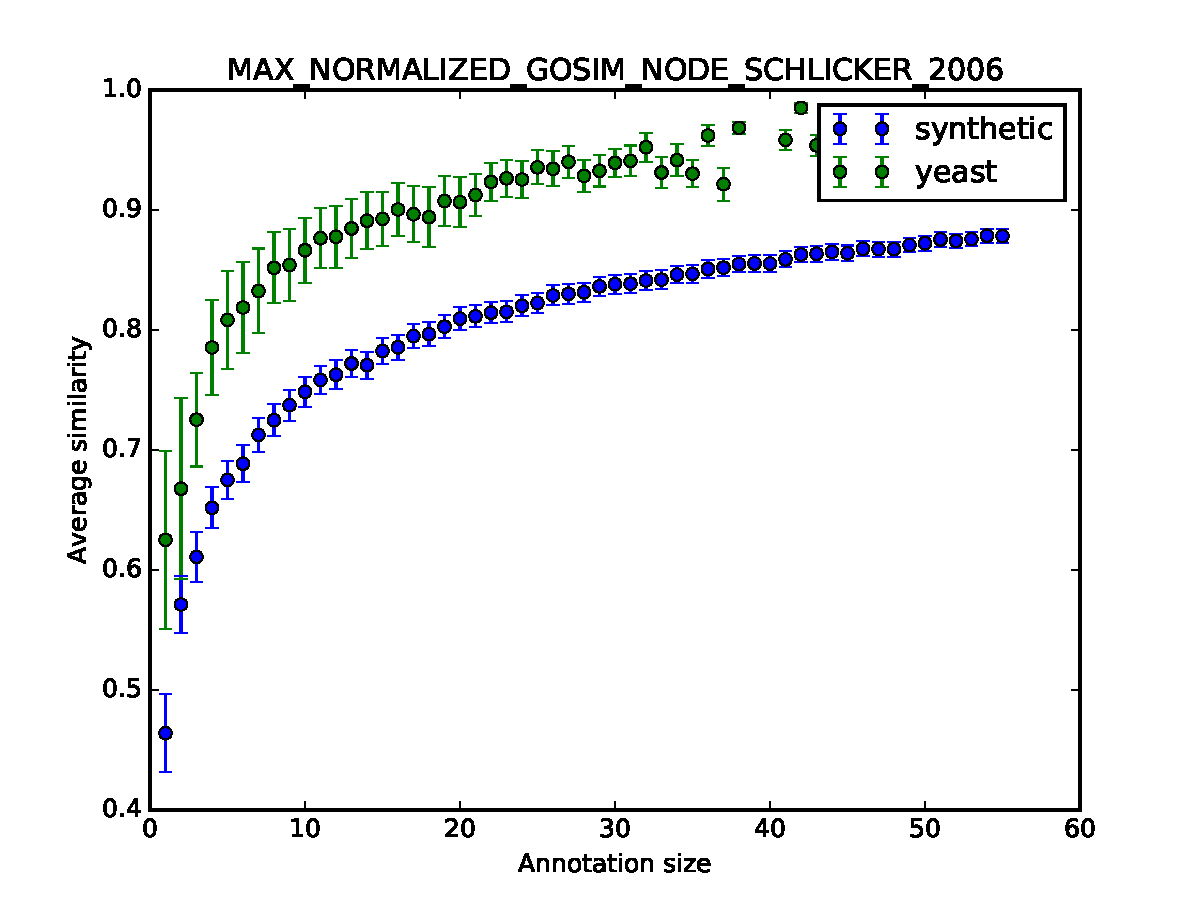
\includegraphics[width=0.5\linewidth, height=0.4\textheight]{pairwise/SIM_GROUPWISE_MAX_NORMALIZED_GOSIM_SIM_PAIRWISE_DAG_NODE_SCHLICKER_2006_avg.pdf}
\end{figure}

\end{frame}

\begin{frame}{Annotation size - Pairwise Similarity Measures}
\begin{figure}
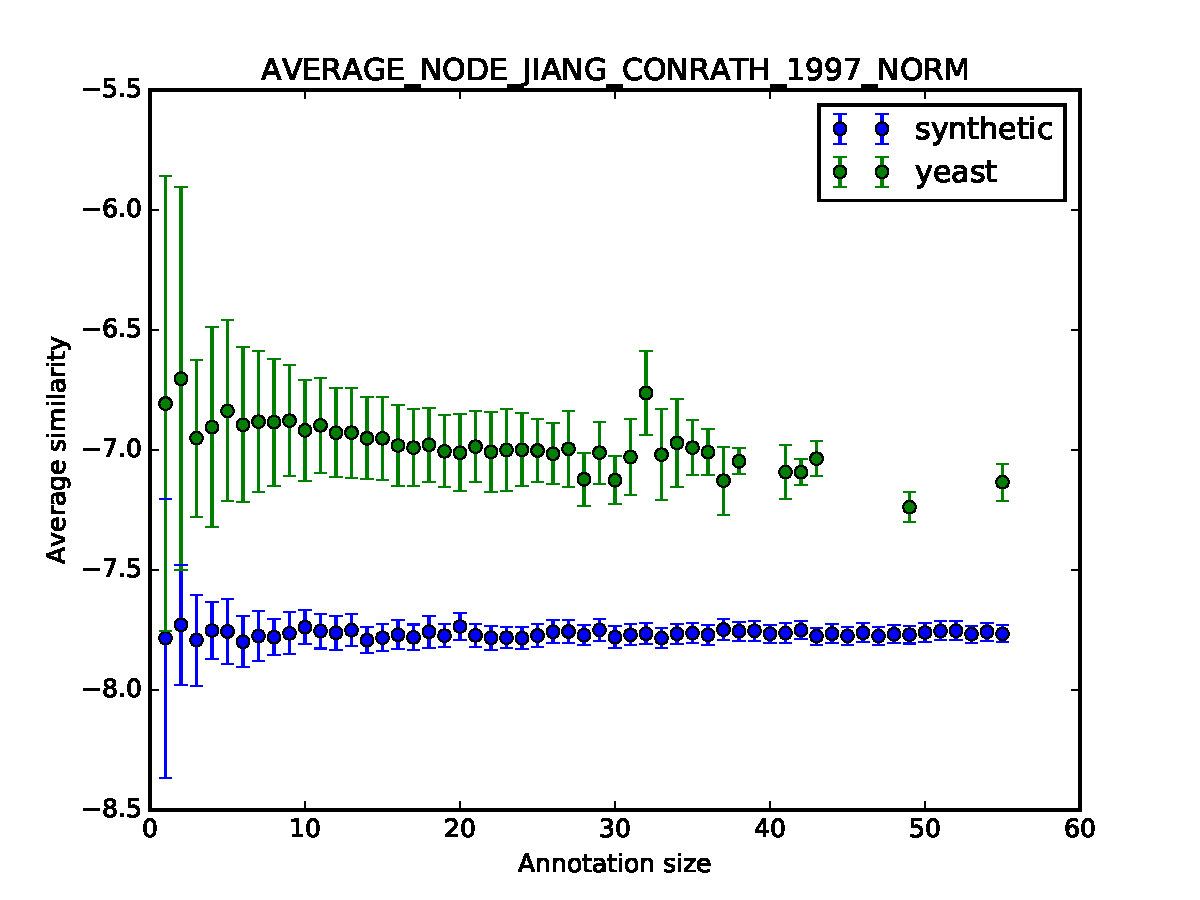
\includegraphics[width=0.5\linewidth, height=0.4\textheight]{pairwise/SIM_GROUPWISE_AVERAGE_SIM_PAIRWISE_DAG_NODE_JIANG_CONRATH_1997_NORM_avg.pdf}
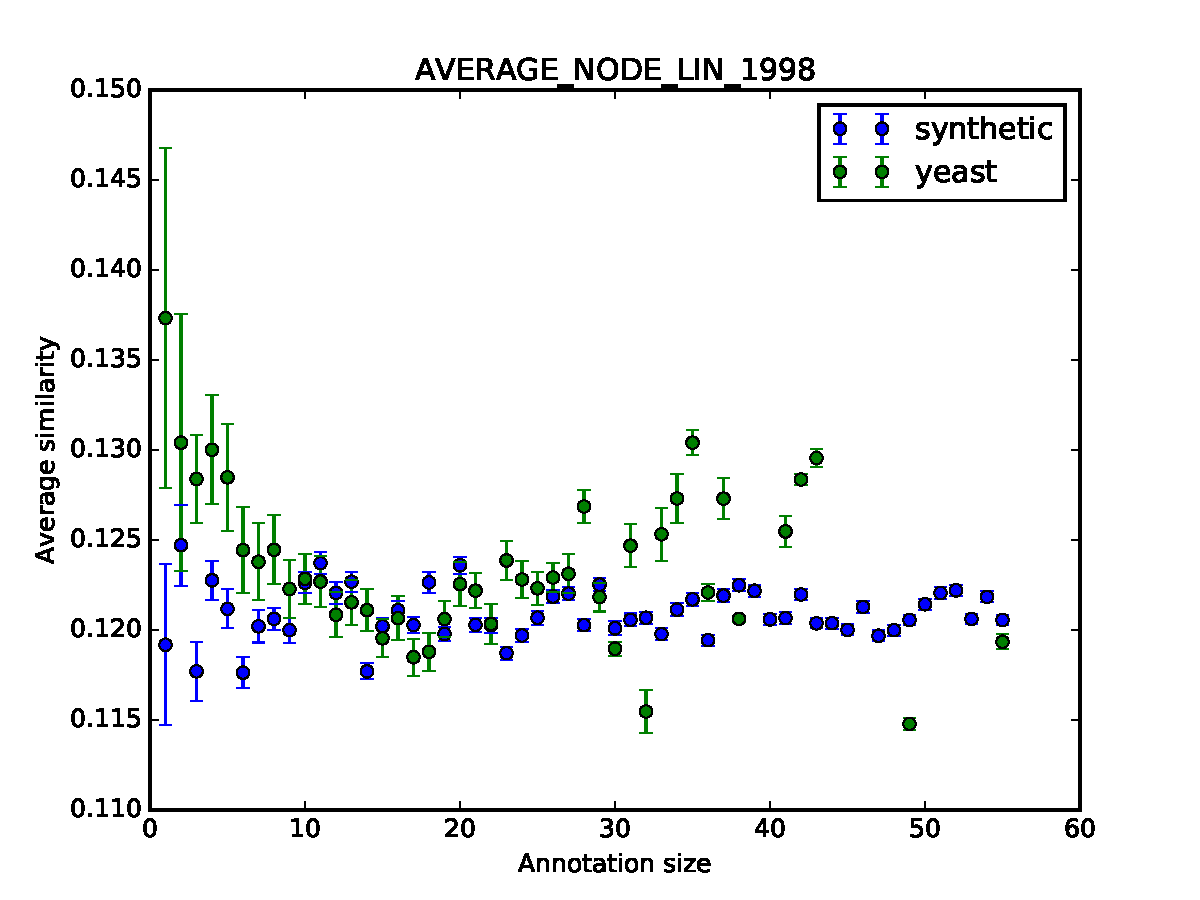
\includegraphics[width=0.5\linewidth, height=0.4\textheight]{pairwise/SIM_GROUPWISE_AVERAGE_SIM_PAIRWISE_DAG_NODE_LIN_1998_avg.pdf} \\
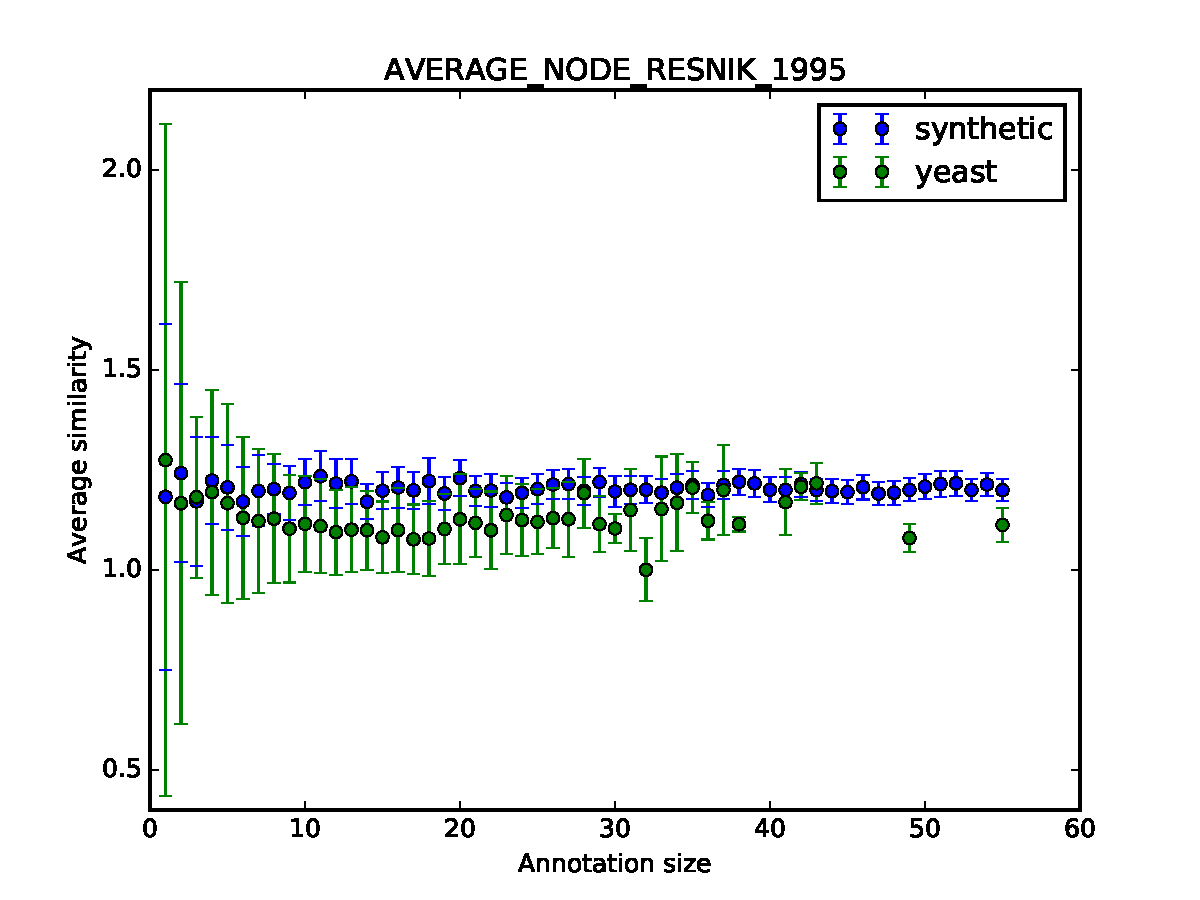
\includegraphics[width=0.5\linewidth, height=0.4\textheight]{pairwise/SIM_GROUPWISE_AVERAGE_SIM_PAIRWISE_DAG_NODE_RESNIK_1995_avg.pdf}
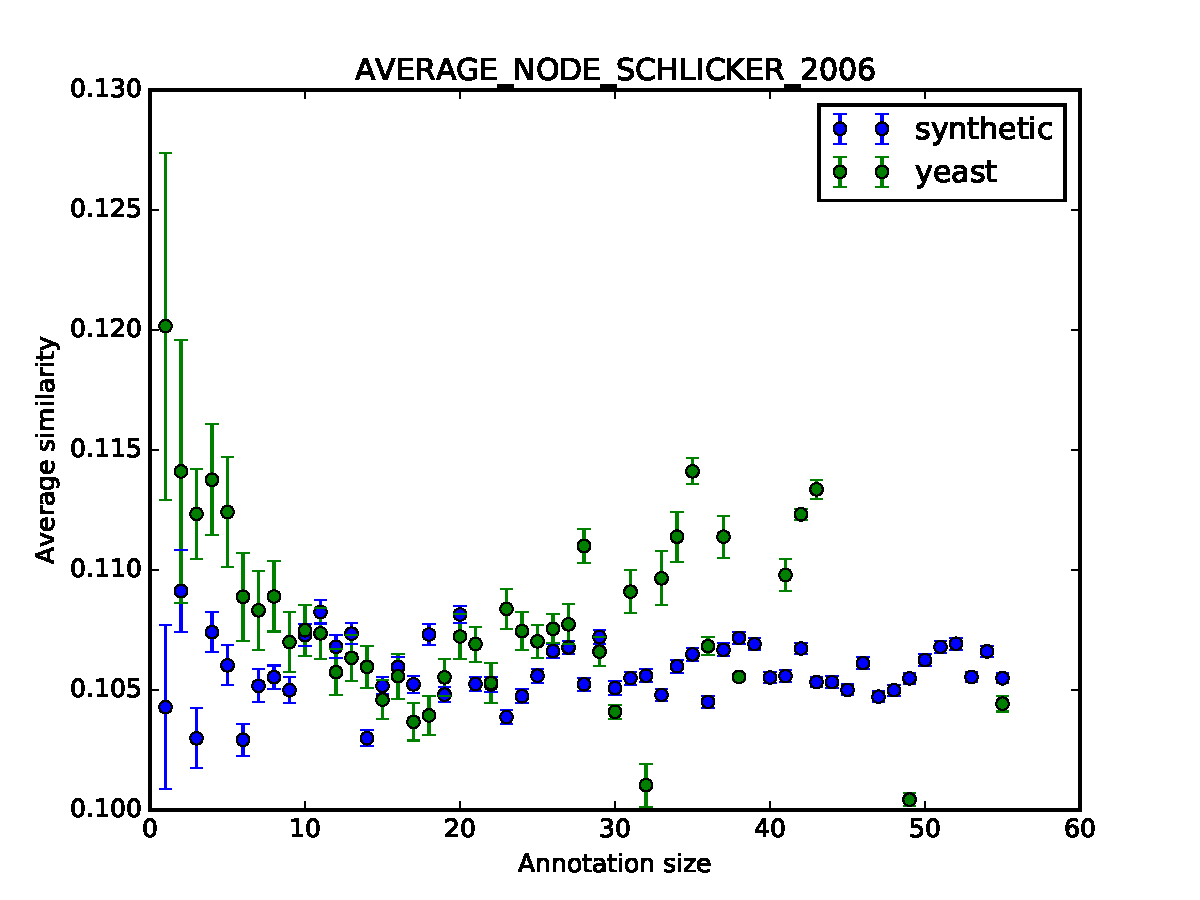
\includegraphics[width=0.5\linewidth, height=0.4\textheight]{pairwise/SIM_GROUPWISE_AVERAGE_SIM_PAIRWISE_DAG_NODE_SCHLICKER_2006_avg.pdf}
\end{figure}
\end{frame}



\begin{frame}{Annotation size difference - Groupwise Similarity Measures}
\begin{figure}
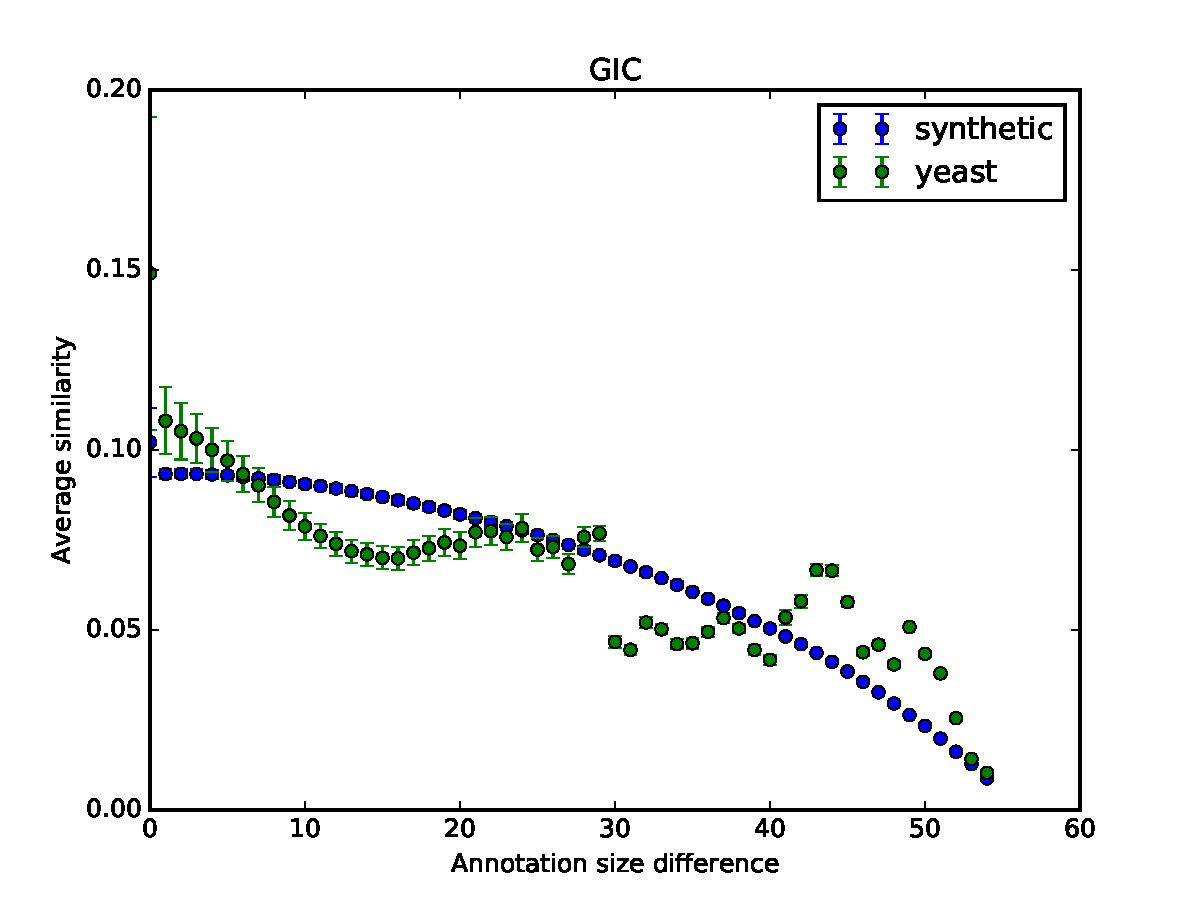
\includegraphics[width=0.5\linewidth, height=0.4\textheight]{groupwise_diff/SIM_GROUPWISE_DAG_GIC_diff.pdf}
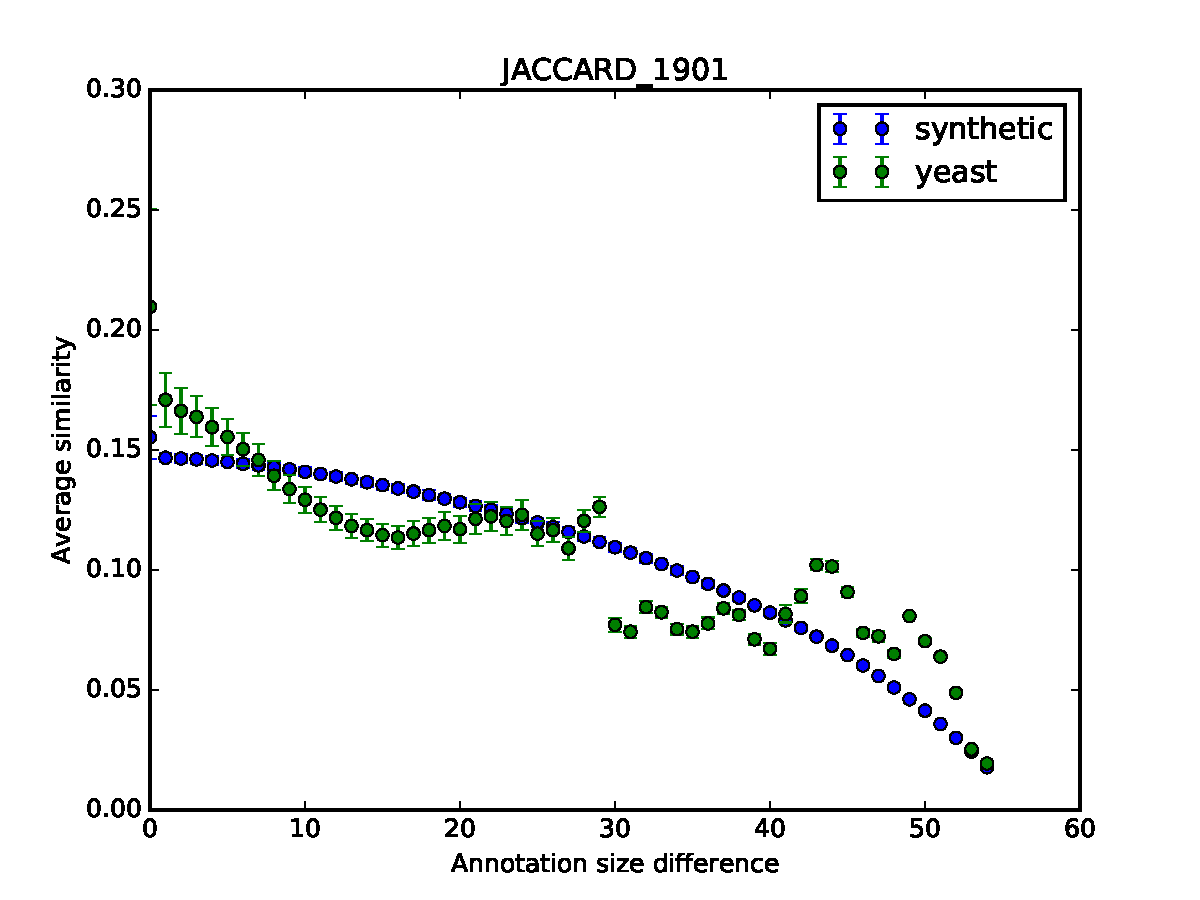
\includegraphics[width=0.5\linewidth, height=0.4\textheight]{groupwise_diff/SIM_FRAMEWORK_DAG_SET_JACCARD_1901_diff.pdf} \\
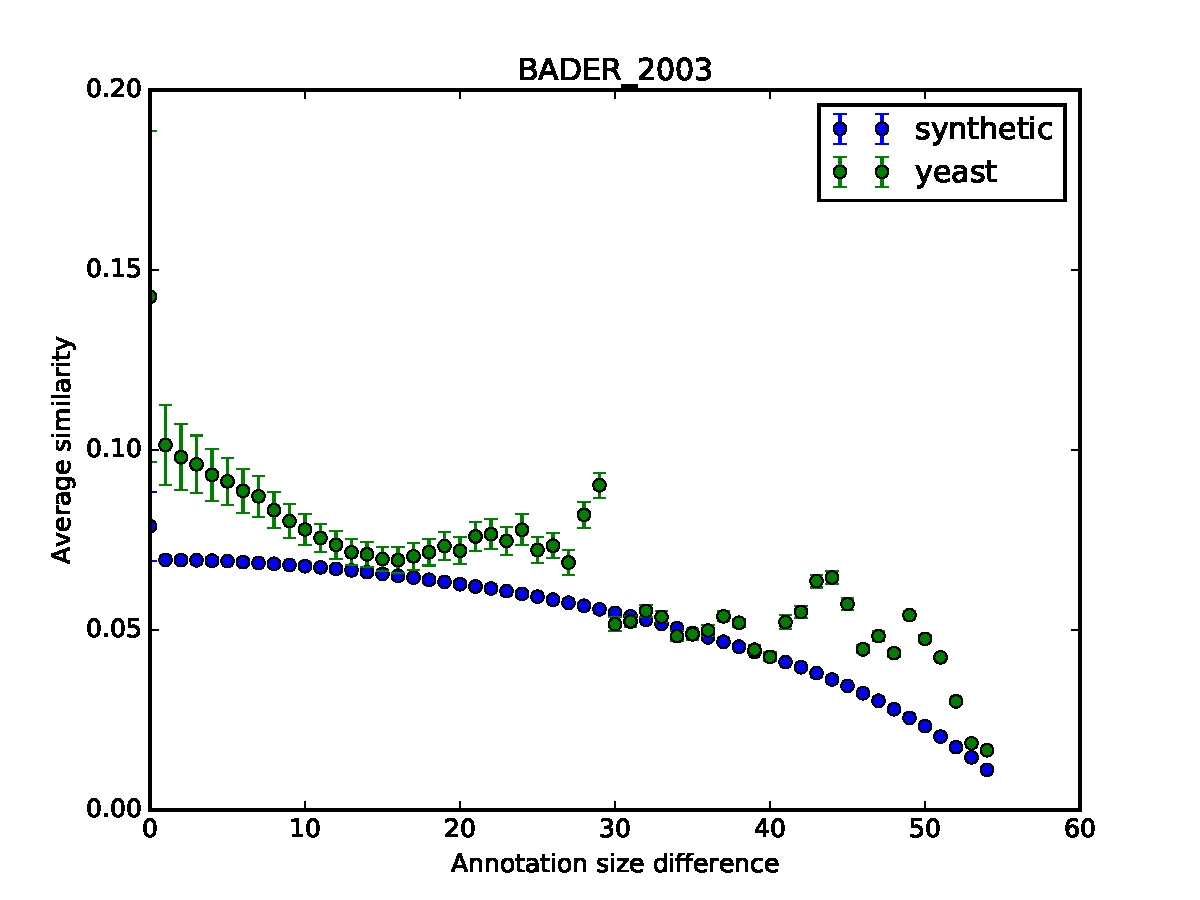
\includegraphics[width=0.5\linewidth, height=0.4\textheight]{groupwise_diff/SIM_FRAMEWORK_DAG_SET_BADER_2003_diff.pdf}
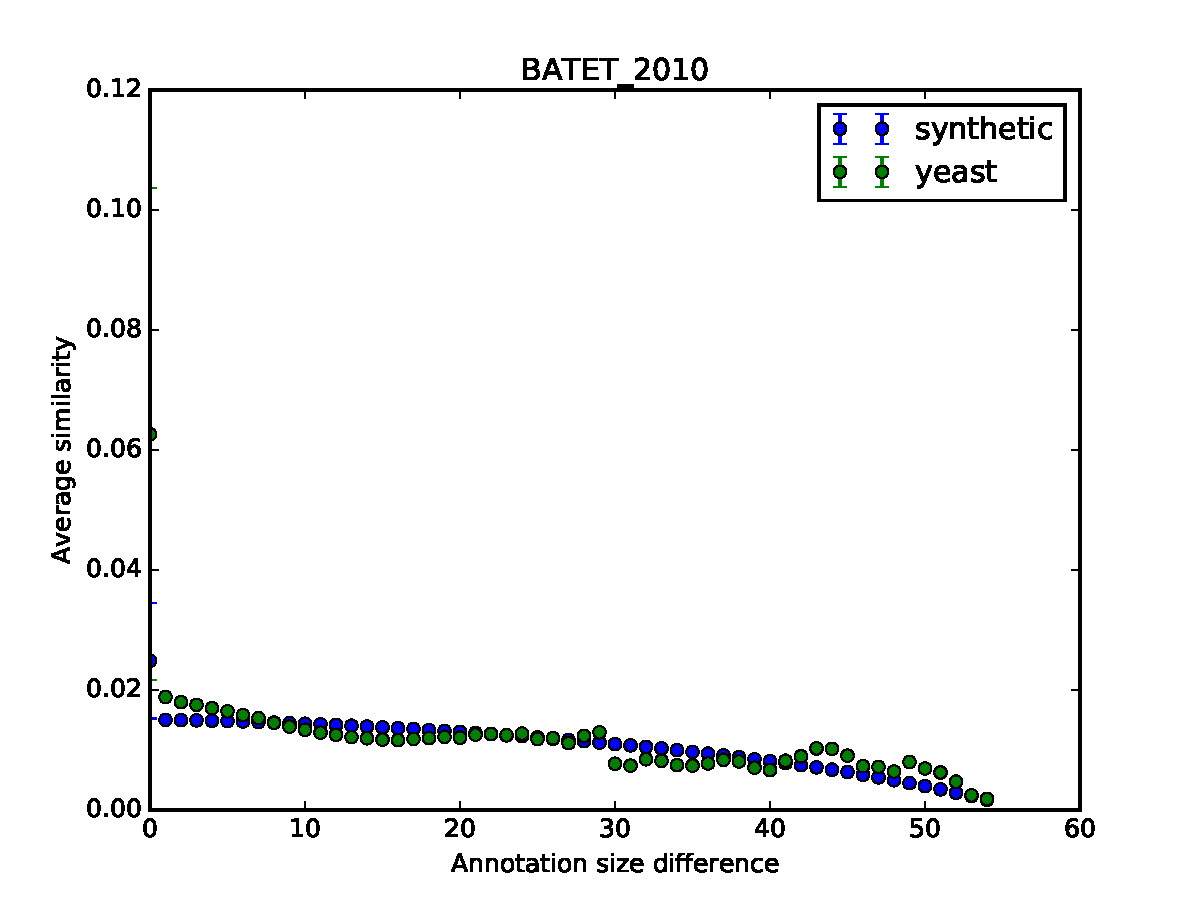
\includegraphics[width=0.5\linewidth, height=0.4\textheight]{groupwise_diff/SIM_FRAMEWORK_DAG_SET_BATET_2010_diff.pdf}
\end{figure}
\end{frame}

\begin{frame}{Annotation size difference - Groupwise Similarity Measures}
\begin{figure}
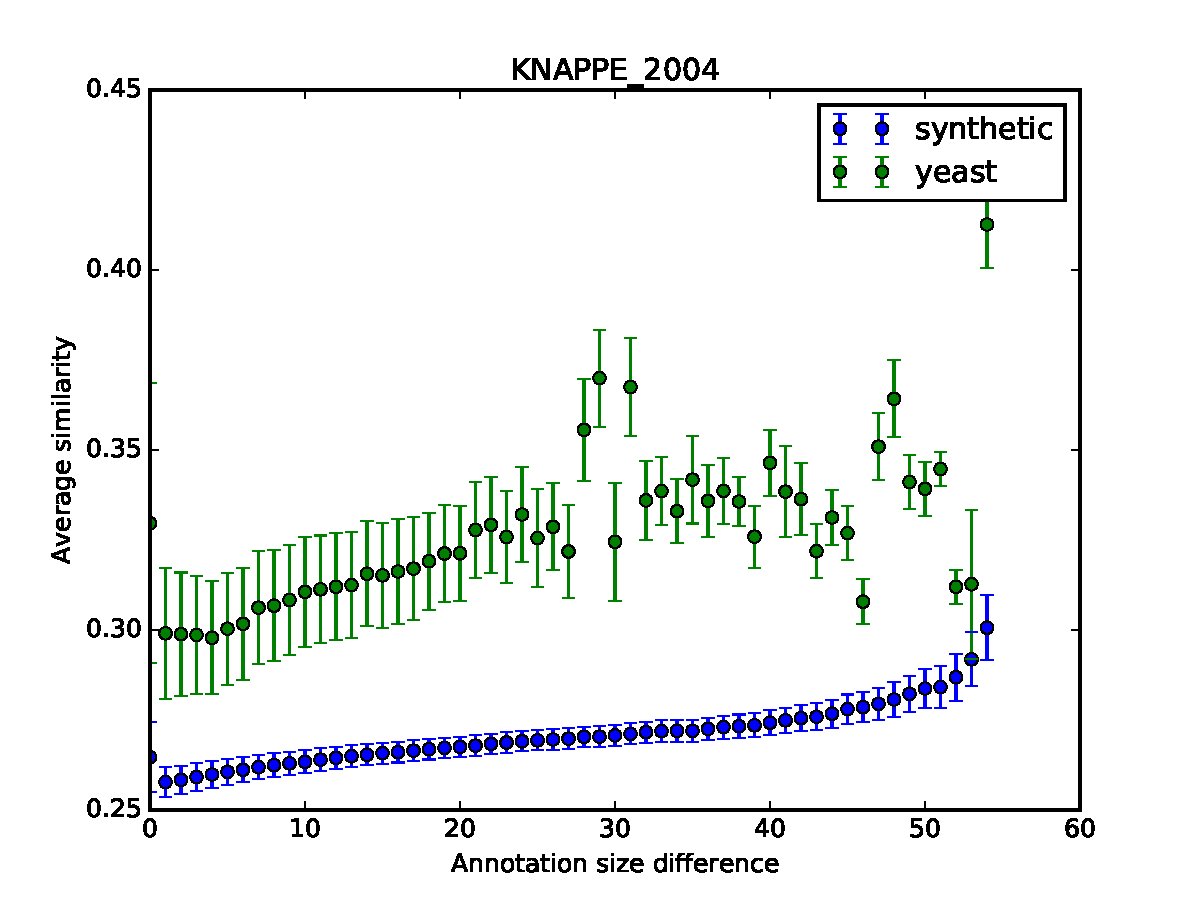
\includegraphics[width=0.5\linewidth, height=0.4\textheight]{groupwise_diff/SIM_FRAMEWORK_DAG_SET_KNAPPE_2004_diff.pdf}
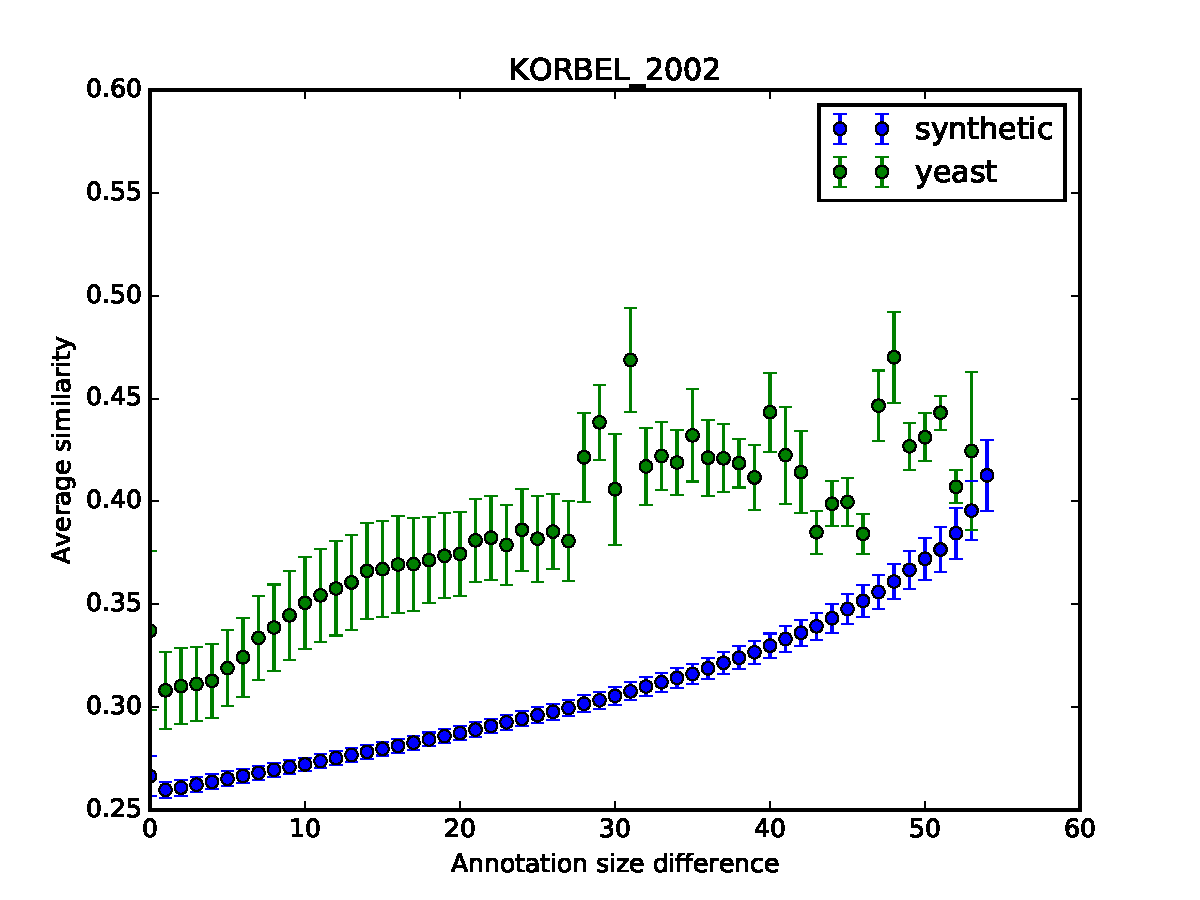
\includegraphics[width=0.5\linewidth, height=0.4\textheight]{groupwise_diff/SIM_FRAMEWORK_DAG_SET_KORBEL_2002_diff.pdf} \\
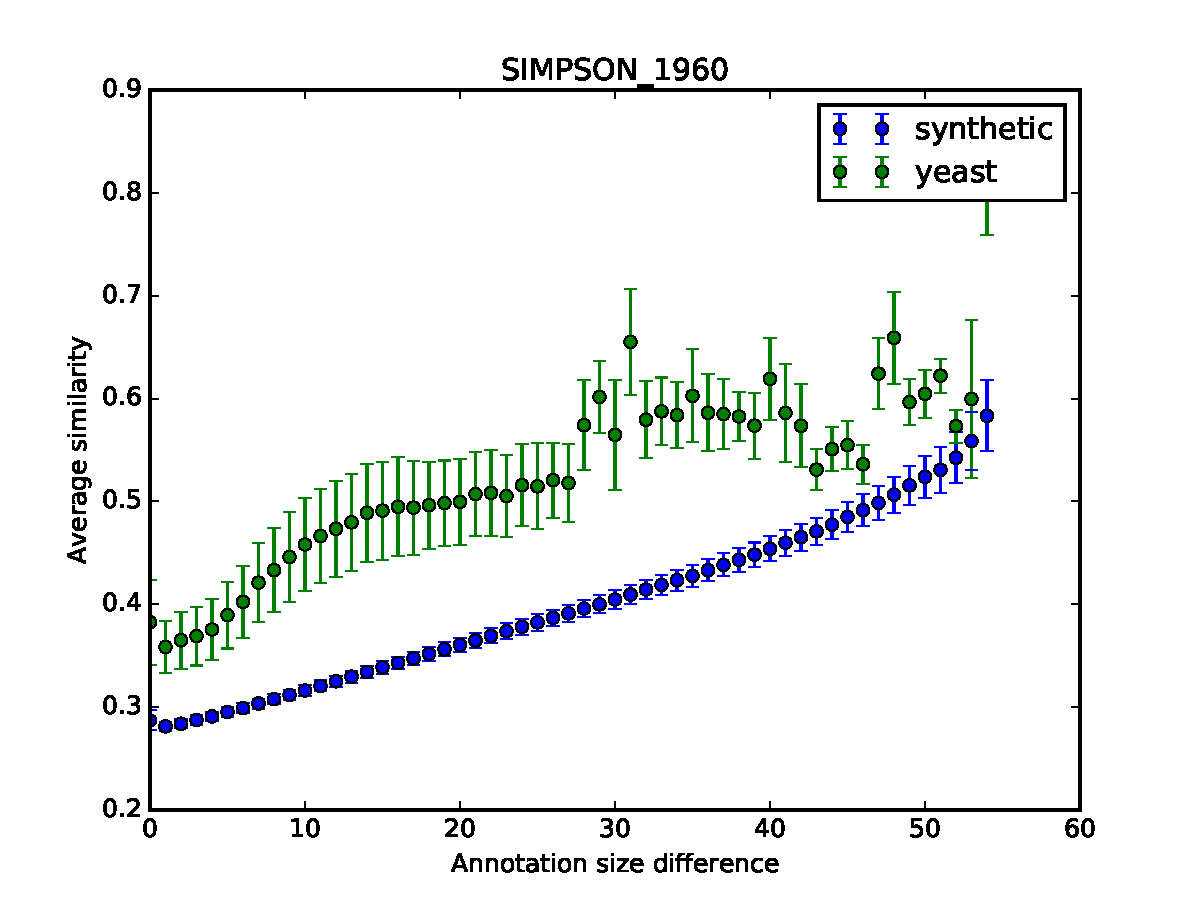
\includegraphics[width=0.5\linewidth, height=0.4\textheight]{groupwise_diff/SIM_FRAMEWORK_DAG_SET_SIMPSON_1960_diff.pdf}
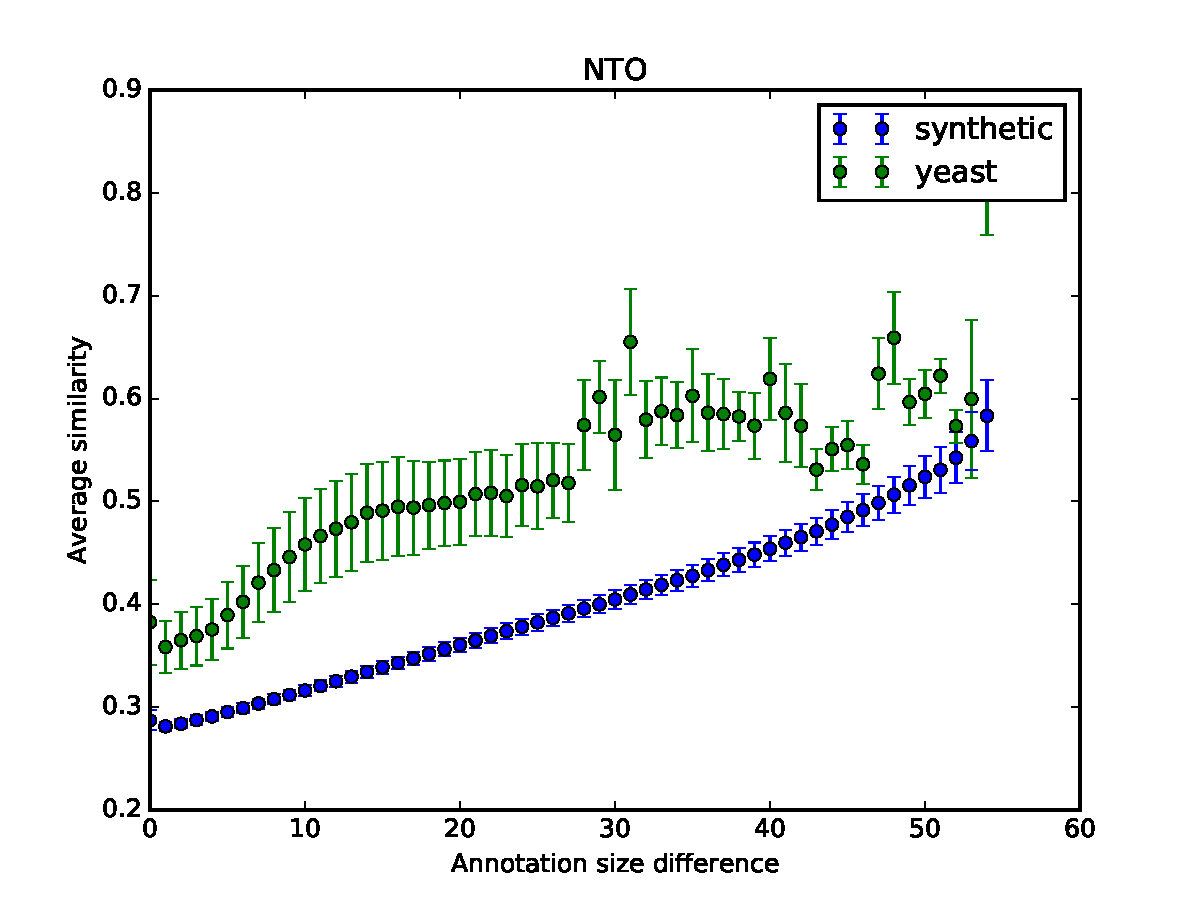
\includegraphics[width=0.5\linewidth, height=0.4\textheight]{groupwise_diff/SIM_GROUPWISE_DAG_NTO_diff.pdf}
\end{figure}
\end{frame}

\begin{frame}{Annotation size difference - Pairwise Similarity Measures}
\begin{figure}
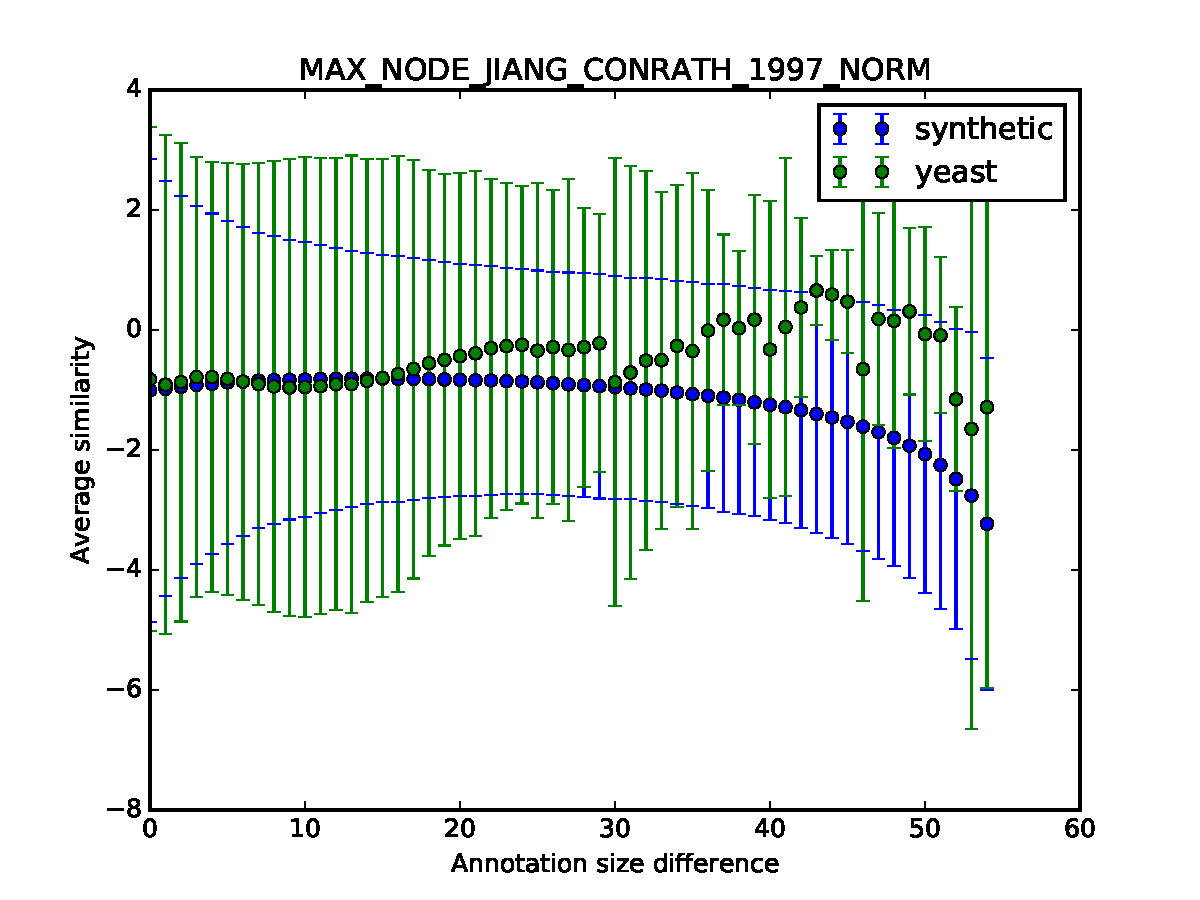
\includegraphics[width=0.5\linewidth, height=0.4\textheight]{pairwise_diff/SIM_GROUPWISE_MAX_SIM_PAIRWISE_DAG_NODE_JIANG_CONRATH_1997_NORM_diff.pdf}
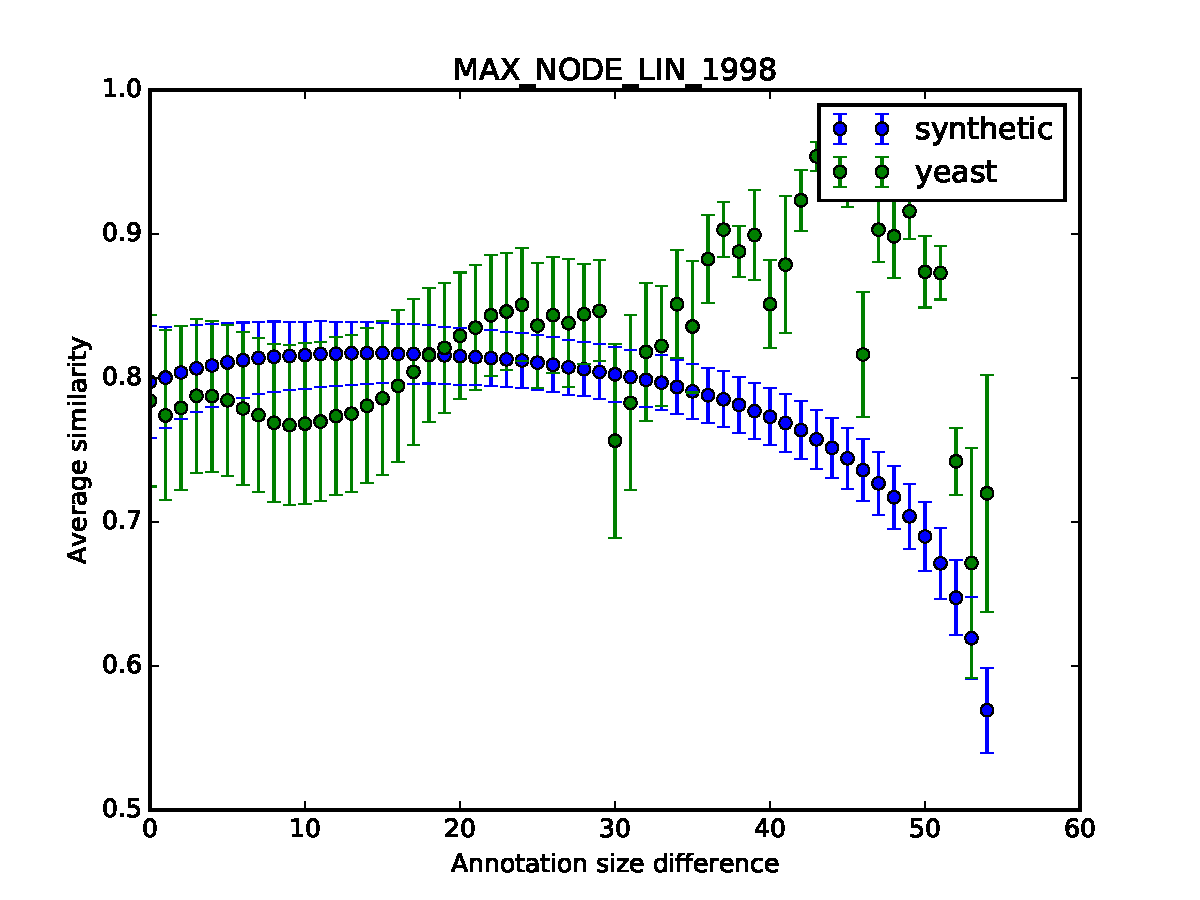
\includegraphics[width=0.5\linewidth, height=0.4\textheight]{pairwise_diff/SIM_GROUPWISE_MAX_SIM_PAIRWISE_DAG_NODE_LIN_1998_diff.pdf} \\
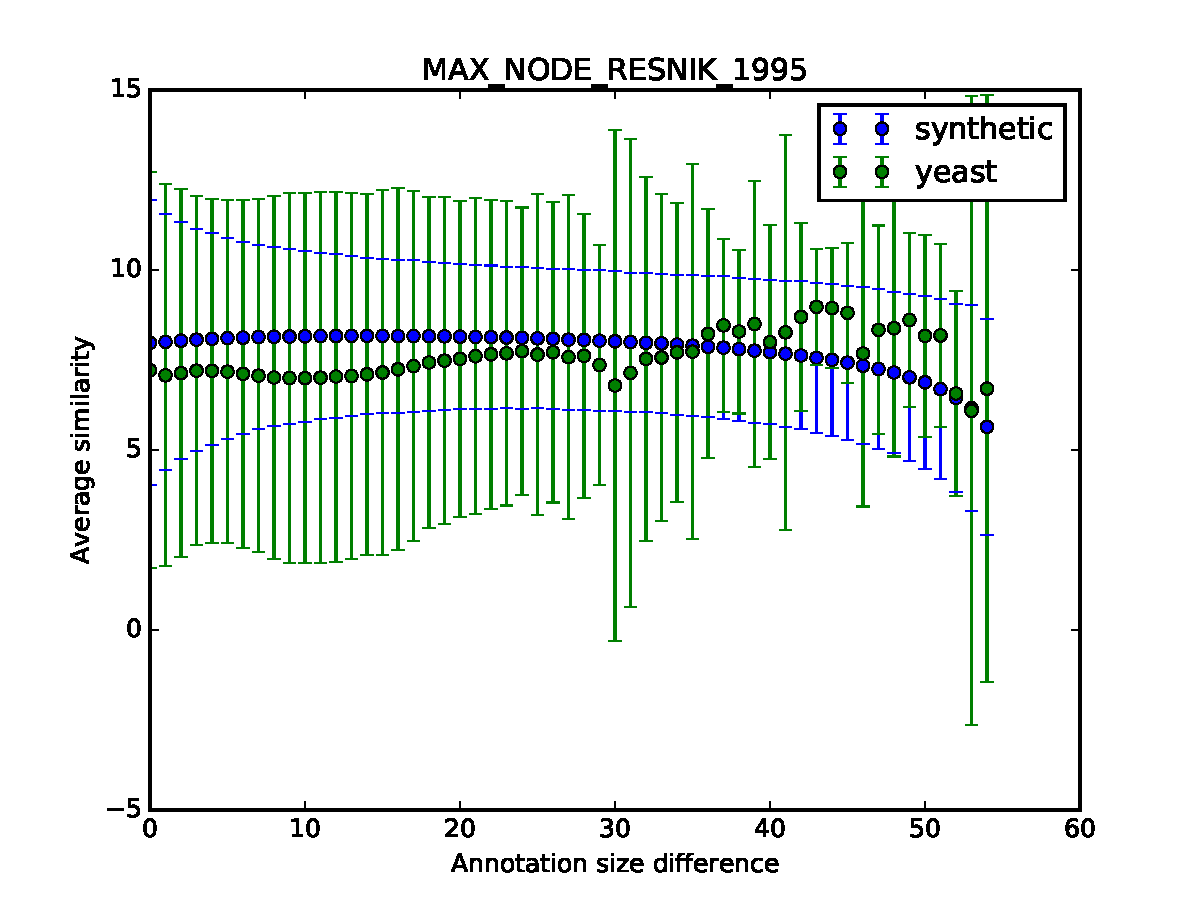
\includegraphics[width=0.5\linewidth, height=0.4\textheight]{pairwise_diff/SIM_GROUPWISE_MAX_SIM_PAIRWISE_DAG_NODE_RESNIK_1995_diff.pdf}
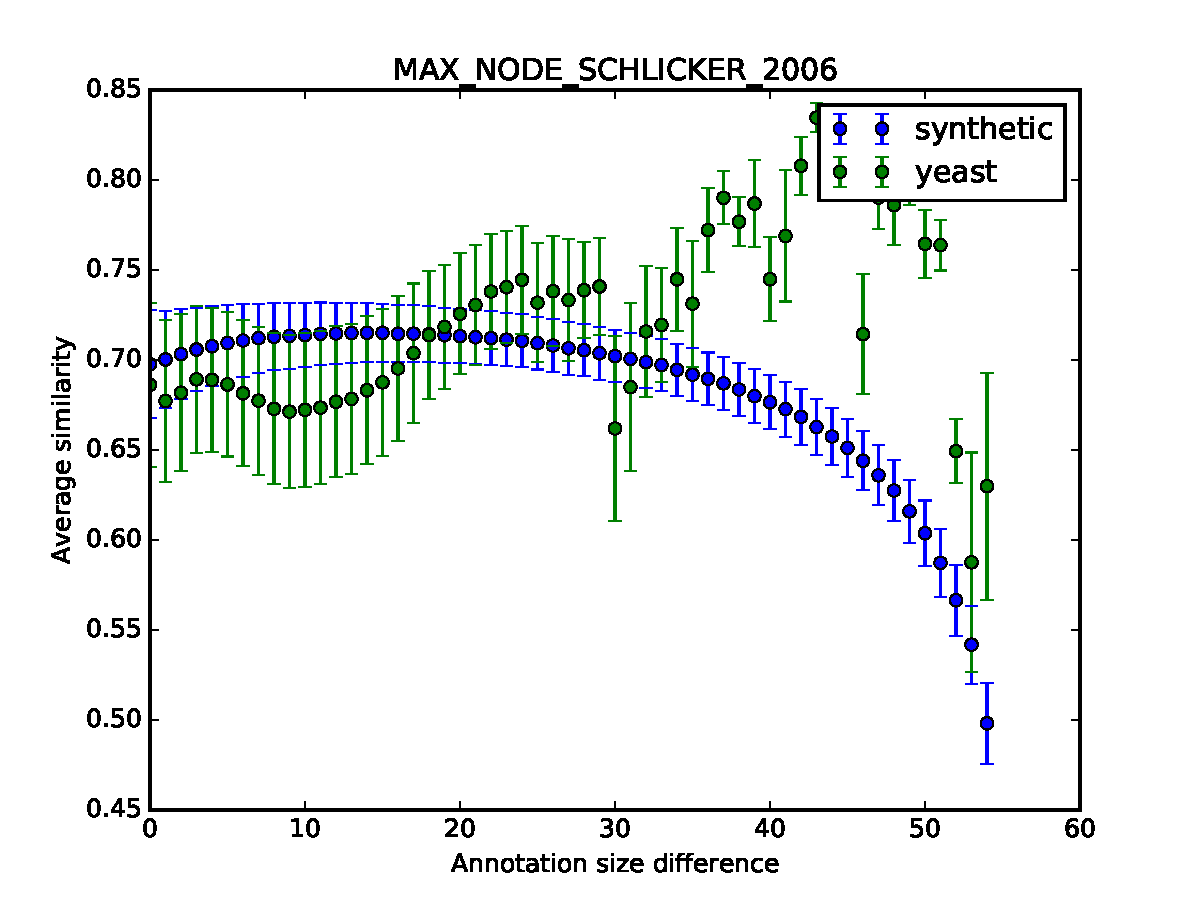
\includegraphics[width=0.5\linewidth, height=0.4\textheight]{pairwise_diff/SIM_GROUPWISE_MAX_SIM_PAIRWISE_DAG_NODE_SCHLICKER_2006_diff.pdf}
\end{figure}
\end{frame}

\begin{frame}{Annotation size difference - Pairwise Similarity Measures}
\begin{figure}
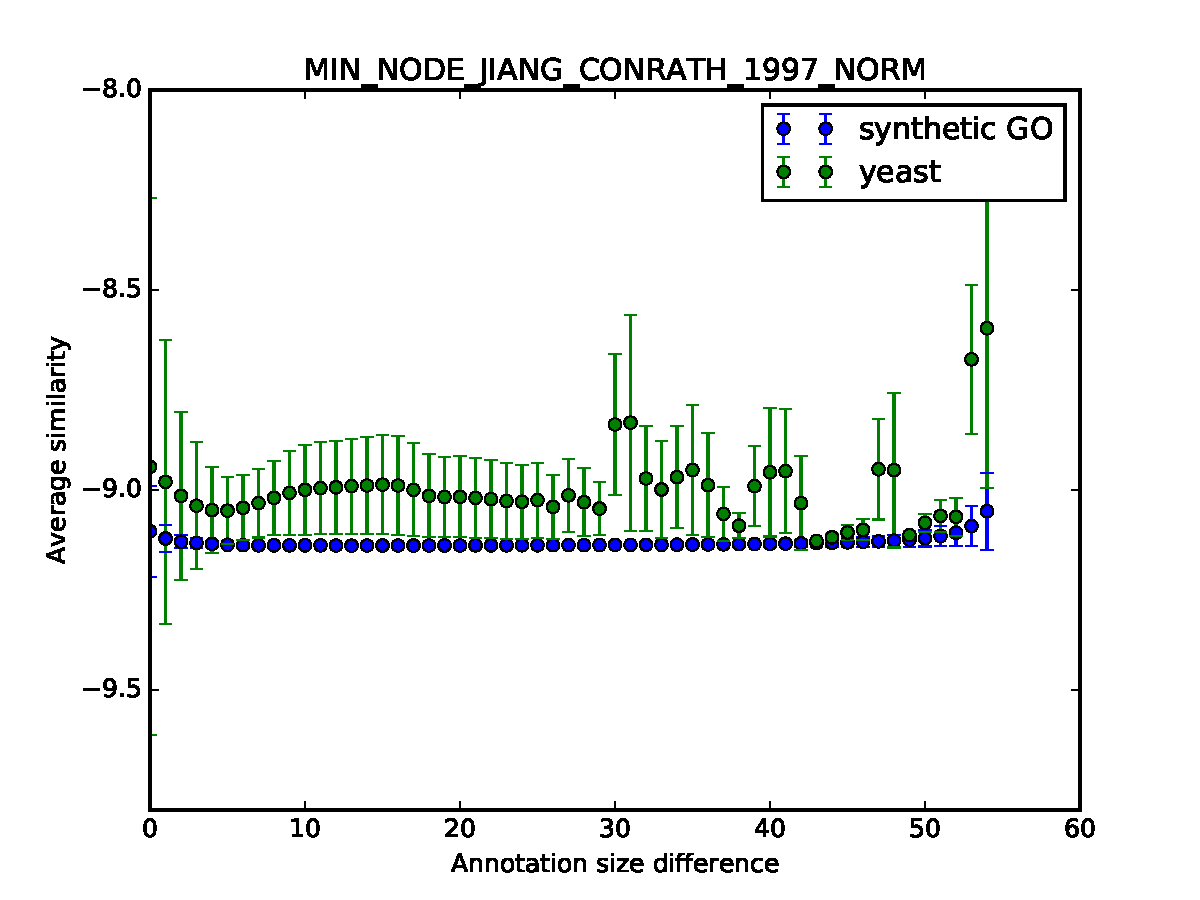
\includegraphics[width=0.5\linewidth, height=0.4\textheight]{pairwise_diff/SIM_GROUPWISE_MIN_SIM_PAIRWISE_DAG_NODE_JIANG_CONRATH_1997_NORM_diff.pdf}
\includegraphics[width=0.5\linewidth, height=0.4\textheight]{pairwise_diff/SIM_GROUPWISE_MIN_SIM_PAIRWISE_DAG_NODE_LIN_1998_diff.pdf} \\
\includegraphics[width=0.5\linewidth, height=0.4\textheight]{pairwise_diff/SIM_GROUPWISE_MIN_SIM_PAIRWISE_DAG_NODE_RESNIK_1995_diff.pdf}
\includegraphics[width=0.5\linewidth, height=0.4\textheight]{pairwise_diff/SIM_GROUPWISE_MIN_SIM_PAIRWISE_DAG_NODE_SCHLICKER_2006_diff.pdf}
\end{figure}
\end{frame}


\begin{frame}{Annotation size difference - Pairwise Similarity Measures}

\begin{figure}

\includegraphics[width=0.5\linewidth, height=0.4\textheight]{pairwise_diff/SIM_GROUPWISE_BMA_SIM_PAIRWISE_DAG_NODE_JIANG_CONRATH_1997_NORM_diff.pdf}
\includegraphics[width=0.5\linewidth, height=0.4\textheight]{pairwise_diff/SIM_GROUPWISE_BMA_SIM_PAIRWISE_DAG_NODE_LIN_1998_diff.pdf}\\
\includegraphics[width=0.5\linewidth, height=0.4\textheight]{pairwise_diff/SIM_GROUPWISE_BMA_SIM_PAIRWISE_DAG_NODE_RESNIK_1995_diff.pdf}
\includegraphics[width=0.5\linewidth, height=0.4\textheight]{pairwise_diff/SIM_GROUPWISE_BMA_SIM_PAIRWISE_DAG_NODE_SCHLICKER_2006_diff.pdf}
\end{figure}

\end{frame}

\begin{frame}{Annotation size difference - Pairwise Similarity Measures}

\begin{figure}
\includegraphics[width=0.5\linewidth, height=0.4\textheight]{pairwise_diff/SIM_GROUPWISE_BMM_SIM_PAIRWISE_DAG_NODE_JIANG_CONRATH_1997_NORM_diff.pdf} 
\includegraphics[width=0.5\linewidth, height=0.4\textheight]{pairwise_diff/SIM_GROUPWISE_BMM_SIM_PAIRWISE_DAG_NODE_LIN_1998_diff.pdf}\\
\includegraphics[width=0.5\linewidth, height=0.4\textheight]{pairwise_diff/SIM_GROUPWISE_BMM_SIM_PAIRWISE_DAG_NODE_RESNIK_1995_diff.pdf}
\includegraphics[width=0.5\linewidth, height=0.4\textheight]{pairwise_diff/SIM_GROUPWISE_BMM_SIM_PAIRWISE_DAG_NODE_SCHLICKER_2006_diff.pdf}
\end{figure}

\end{frame}

\begin{frame}{Annotation size difference - Pairwise Similarity Measures}
\begin{figure}
\includegraphics[width=0.5\linewidth, height=0.4\textheight]{pairwise_diff/SIM_GROUPWISE_MAX_NORMALIZED_GOSIM_SIM_PAIRWISE_DAG_NODE_JIANG_CONRATH_1997_NORM_diff.pdf}
\includegraphics[width=0.5\linewidth, height=0.4\textheight]{pairwise_diff/SIM_GROUPWISE_MAX_NORMALIZED_GOSIM_SIM_PAIRWISE_DAG_NODE_LIN_1998_diff.pdf} \\
\includegraphics[width=0.5\linewidth, height=0.4\textheight]{pairwise_diff/SIM_GROUPWISE_MAX_NORMALIZED_GOSIM_SIM_PAIRWISE_DAG_NODE_RESNIK_1995_diff.pdf}
\includegraphics[width=0.5\linewidth, height=0.4\textheight]{pairwise_diff/SIM_GROUPWISE_MAX_NORMALIZED_GOSIM_SIM_PAIRWISE_DAG_NODE_SCHLICKER_2006_diff.pdf}
\end{figure}
\end{frame}

\begin{frame}{Annotation size difference - Pairwise Similarity Measures}
\begin{figure}
\includegraphics[width=0.5\linewidth, height=0.4\textheight]{pairwise_diff/SIM_GROUPWISE_AVERAGE_NORMALIZED_GOSIM_SIM_PAIRWISE_DAG_NODE_JIANG_CONRATH_1997_NORM_diff.pdf}
\includegraphics[width=0.5\linewidth, height=0.4\textheight]{pairwise_diff/SIM_GROUPWISE_AVERAGE_NORMALIZED_GOSIM_SIM_PAIRWISE_DAG_NODE_LIN_1998_diff.pdf} \\
\includegraphics[width=0.5\linewidth, height=0.4\textheight]{pairwise_diff/SIM_GROUPWISE_AVERAGE_NORMALIZED_GOSIM_SIM_PAIRWISE_DAG_NODE_RESNIK_1995_diff.pdf}
\includegraphics[width=0.5\linewidth, height=0.4\textheight]{pairwise_diff/SIM_GROUPWISE_AVERAGE_NORMALIZED_GOSIM_SIM_PAIRWISE_DAG_NODE_SCHLICKER_2006_diff.pdf}
\end{figure}
\end{frame}

\begin{frame}{Annotation size difference - Pairwise Similarity Measures}
\begin{figure}
\includegraphics[width=0.5\linewidth, height=0.4\textheight]{pairwise_diff/SIM_GROUPWISE_AVERAGE_SIM_PAIRWISE_DAG_NODE_JIANG_CONRATH_1997_NORM_diff.pdf}
\includegraphics[width=0.5\linewidth, height=0.4\textheight]{pairwise_diff/SIM_GROUPWISE_AVERAGE_SIM_PAIRWISE_DAG_NODE_LIN_1998_diff.pdf} \\
\includegraphics[width=0.5\linewidth, height=0.4\textheight]{pairwise_diff/SIM_GROUPWISE_AVERAGE_SIM_PAIRWISE_DAG_NODE_RESNIK_1995_diff.pdf}
\includegraphics[width=0.5\linewidth, height=0.4\textheight]{pairwise_diff/SIM_GROUPWISE_AVERAGE_SIM_PAIRWISE_DAG_NODE_SCHLICKER_2006_diff.pdf}
\end{figure}
\end{frame}

%-----------------------------------------------

\begin{frame}{Summary}
\begin{itemize}
\item Most of the similarity measures are sensitive to the annotation size
\item Pairwise measures depend on combination
\item Well annotated entities get higher similarities
\item Studies which use similarity measures may be biased by annotation size
\end{itemize}
\end{frame}

%-----------------------------------------------

\begin{frame}{Protein-protein interaction predictions}
\begin{figure}
\includegraphics[width=0.5\linewidth, height=0.4\textheight]{ppi/figure_gic_yeast.eps}
\includegraphics[width=0.5\linewidth, height=0.4\textheight]{ppi/figure_gic_random.eps} \\
\includegraphics[width=0.5\linewidth, height=0.4\textheight]{ppi/figure_bma_resnik_yeast.eps}
\includegraphics[width=0.5\linewidth, height=0.4\textheight]{ppi/figure_bma_resnik_random.eps}
\end{figure}
\end{frame}

%-----------------------------------------------

\begin{frame}{Protein-protein interaction predictions}
\begin{figure}
\includegraphics[width=0.5\linewidth, height=0.5\textheight]{ppi/figure_average_resnik_yeast.eps}
\includegraphics[width=0.5\linewidth, height=0.5\textheight]{ppi/figure_average_resnik_random.eps}
\end{figure}
\end{frame}

%-----------------------------------------------

\begin{frame}{Recommendations}
\begin{itemize}
\item If annotations size variance is high, use pairwise similarity measures with average strategy
\end{itemize}
\end{frame}

%------------------------------------------------

\begin{frame}
\Huge{\centerline{Thanks!}}
\small{\centerline{\url{http://www.cbrc.kaust.edu.sa/onto/sim-eval/}}}
\end{frame}

%----------------------------------------------------------------------------------------

\end{document}